\documentclass[%
 %reprint, %uncomment to make into two columns
%superscriptaddress,
%groupedaddress,
%unsortedaddress,
%runinaddress,
%frontmatterverbose, 
% preprint, %comment to make into two columns
%showpacs,preprintnumbers,
%nofootinbib,
%nobibnotes,
%bibnotes,
 amsmath,amssymb,
 aps,
 prc
%pra,
%prb,cms@ex
%rmp,
%prstab,
%prstper,
%floatfix,
]{revtex4-1}
\usepackage[compat=1.0.0]{tikz-feynman}
\usepackage{graphicx}% Include figure files
\usepackage{graphics}
\usepackage{ctable}
\usepackage{dcolumn}% Align table columns on decimal point
\usepackage{bm}% bold math
\usepackage{ifthen}
\usepackage{xspace}
%\usepackage{ptdr-definitions}
\usepackage{rotating}
%number the lines
\usepackage{lineno,xcolor}
% Running line numbers:
%\linenumbers
\setlength\linenumbersep{5pt}
\usepackage{setspace}
\linespread{1.3} %1.3 by default
\newboolean{cms@external}
\setboolean{cms@external}{true}
\usepackage{amsfonts}
\usepackage{booktabs}
\usepackage{siunitx}
\usepackage{capt-of}
\usepackage{color}

\newcommand{\blue}{\color{blue}}
\newcommand{\green}{\color{green}}
\newcommand{\red}{\color{red}}
\newcommand{\magenta}{\color{magenta}}
\newcommand{\cyan}{\color{cyan}}
\newcommand{\sm}{\footnotesize}

\usepackage{feynmp-auto}
%\usepackage{hyperref}% add hypertext capabilities
%\usepackage[mathlines]{lineno}% Enable numbering of text and display math
%\linenumbers\relax % Commence numbering lines

%\usepackage[showframe,%Uncomment any one of the following lines to test 
%%scale=0.7, marginratio={1:1, 2:3}, ignoreall,% default settings
%%text={7in,10in},centering,
%%margin=1.5in,
%%total={6.5in,8.75in}, top=1.2in, left=0.9in, includefoot,
%%height=10in,a5paper,hmargin={3cm,0.8in},
%]{geometry}

%------------------------------------------------------------

\begin{document}



\title{Study of WW $\rightarrow q\bar{q}\ell\bar{\nu}$ at ILC500 with ILD }
\author{Justin Anguiano}
\date{\today}

%------------------------------------------------------------

\begin{abstract}
%\documentclass[11pt,a4paper]{article}
%\usepackage[utf8]{inputenc}
%\usepackage{amsmath}
%\usepackage{amsfonts}
%%\usepackage{amssymb}
%\begin{document}

%\end{document}

The work presented is an analysis for detector R\&D at the International Linear Collider(ILC). The study showcases the approaches towards lepton identification and pileup mitigation at center-of-mass energy $\sqrt{s} = 500$ GeV for the semileptonic WW process. The analysis is performed using fully simulated Standard Model Monte Carlo events and emphasizes the measurement of the W mass. The mass measurement is performed through the identification of a lepton and treatment of the remaining system as the hadronic W-boson within the most favorable beam polarization scenario for WW production. The resulting detector performance benchmark with an integrated luminosity of $1600 \, \, \text{fb}^{-1}$ is the statistical error on the W mass $\Delta M_W =  2.4 $ MeV and a relative statisical error on the WW cross-section $\Delta \sigma / \sigma = 0.04 \% $


\end{abstract}

%------------------------------------------------------------

\maketitle

%------------------------------------------------------------

\section{Introduction and motivation}
\label{sec:Introduction}
%The W-boson pair decaying semileptonically is a rich physics channel with a wide varietey of facets to study. The most well motivated is the measurement of the W mass because of the easy identification of the lepton which automatically tags the hadronic W as the remaining particles in the system. The mass measurement quality is then only bounded by the performance of the detector. WW production is also sensitive to the polarization of electron positron collider beams.  Measuring the production cross section  implicity measures the beam polarization at the interaction point. Another important aspect of WW, is the charged triple gauge couplings(TGCs). Deviation of these couplings with the Standard Model is a distinct signature of new physics. This study assesses the challenges associated with reconstruction and analysis of semileptonic W pairs at center of mass energy 500 GeV, which is important tool in understanding the problems that lie in analysis within the next frontier of particle physics. The work presented contains four major steps. The first step is the identification of the lepton, which is done with a universal treatment of leptons, that is, nwithout distinguishing between types of leptons.  Second, the effects of pileup on the hadronic mass are explored and a technique to reduce this effect is showcased. Third is the event selection where W pairs are selected against the full standard model background. Lastly, measurements for the statiscal error of the W mass and cross section are extracted.

\section{Physics}
\label{sec:physics}
%\subsection{Standa physics}
%\label{subsec:ElectorWeak_physics}

\subsection{The Standard Model}
\label{subsec:std_model}
The current standard model consists of two types of elementary particles: fermions and bosons. The fermions have a half-integer spin (1/2) and can be further separated into two categories: quarks and leptons. The quarks have three known generations, the first being the light quarks up(u) and down(d), the next generation gets increasingly more massive with the charm(c) and strange(s) quarks, and the most massive generation consists of the top(t) and bottom(b) quarks. Each individaul quark also carries a fractional electrical charge of either $+2/3$ for the uplike quarks (u,c,t)  or $-1/3$ for the downlike quarks (d,s,b). The charged leptons are also comprised of three generations of increasing mass, they are the electron($e$), muon($\mu$), and tau($\tau$). Each charged lepton is accompanied by neutrally charged  neutrino $\nu_e , \, \nu_\mu , \, \nu_\tau$. Bosons can be subdivided into two groups as well, the vector bosons and scalar boson. The singular scalar boson is the spin 0 Higgs Boson,  responsible for giving particles mass. There are four known vector bosons the photon($\gamma$), gluon($g$), $W^\pm$, and $Z^0$.  Each  vector boson has a spin of 1 and each governs specific interactions between particles. The most well known boson is the photon, the photon mediates interaction between particles which have charge.The gluon mediates the strong force and is responsible for the interactions between quarks. The W and Z bosons are the mediators of the weak force and the only known particles that interact with neutrinos.

--- \textit{The W-boson }\\
 The W boson is electrically charged where as its partner the Z is electrically neutral. The W boson decays through a flavor changing vertex, meaning that the particles involved in the decay vertex are always different flavors, and often the same generation, as long as charge and lepton number is conserved. Examples of the W fundamental vertices coupling with fermions is shown in Figure \ref{fig:verts}. The rate at which the W decays hadronically(to a pair of quarks) or Branching Ratio(BR) is $\approx 70\%$. The rate at which a charged lepton and neutrino is produced is $\approx30\%$ and is split approximately evenly between the three charged leptons. The most difficult reconstruction of a final state from W decay is the case of a tau lepton. The tau can mimic the signature of hadrons or other leptons in a detector in addition to producing additional missing energy via neutrinos. The tau has a shorter lifetime compared to the other charged leptons and flies a short distance before decaying. If produced from the interaction point in a detector, the tau will travel on average $8\,\mu\text{m}$ before decaying. The other leptons, like the electron, is stable and doesn't decay, and the muon is not stable but is unlikely to decay inside of the detector. The tau lepton mainly decays hadronically -- into a tau neutrino and virtual W-boson that produces a pair of quarks. The virtual W's daughter quarks will hadronize into a charged particle ($\pi^\pm$) or radiate more quarks that form either more charged or neutral particles ($\pi^0$). If $\pi^0$'s are created they immediately decay into two photons. When a tau produces a single charged particle this is classified as a 1-prong decay, 3 charged particles is classified as a 3-prong decay. The virtual W in the tau decay is allowed to decay into leptons, so, the tau final state can include either a electron or muon along with the corresponding flavor neutrinos. The decay rates for tau are given in Table \ref{tab:taudecay}.

\begin{table}[h] 

 \parbox{249pt}{
    \begin{minipage}{0.45\textwidth}
        \centering
 \begin{tabular}{|c|l|c|} \toprule
 \hline
       & Decay Mode & Branching Ratio  \\ \hline \hline
    Hadronic Modes  & $\pi^- \nu_\tau$  & $10.82\%$  \\
      	($64.79\%$) & $\pi^- \pi^0 \nu_\tau$ & $25.49\%$ \\
     				& $\pi^- \pi^0 \pi^0 \nu_\tau$  & $9.26\%$  \\
     				& $\pi^- \pi^0 \pi^0 \pi^0 \nu_\tau$  & $1.04\%$   \\
      				& $\pi^- \pi^+ \pi^- \nu_\tau$  & $8.99\%$      \\ \midrule
      				& $\pi^- \pi^+ \pi^- \pi^0 \nu_\tau$  & $2.74\%$  \\ \hline
    			    
    Leptonic Modes  & $e^- \nu_e \nu_\tau$ & $17.82\%$   \\
    	($35.21\%$)	& $\mu^- \nu_\mu \nu_\tau $  & $17.39\%$      \\ \midrule \hline
      				
     				
\end{tabular}
        \caption{\label{tab:taudecay}Most common decay modes for the $\tau^-$ lepton \cite{pdg}}

       
  
    \end{minipage}\hfill

   }
   \parbox{249pt}{

    \begin{minipage}{0.45\textwidth}
        \centering
        \feynmandiagram [horizontal=a to b] {
  
  a -- [photon, edge label=\(  W^{+}\)] b,
  f1 [particle=\(u\)] -- [fermion] b -- [fermion] f2 [particle=\(\bar{s}\)],
};
    \feynmandiagram[horizontal=a to b ]{
        a -- [photon, edge label=\(  W^{-}\)] b,
  f1 [particle=\(\mu^{-}\)] -- [fermion] b -- [fermion] f2 [particle=\(\bar{\nu_{\mu}}\)],
    };
    	%\caption{Fundamental vertices between the W-boson and fermions }
        %\includegraphics[width=0.9\textwidth]{example-image-b} % second figure itself
       % \caption{second figure}
       \captionof{figure}{Fundamental vertices between the W-boson and fermions}
       \label{fig:verts}
    \end{minipage}
}
\end{table}

--- \textit {The W Mass}\\
The W-boson is an unstable particle and abides by a total decay rate $\Gamma = 1/\tau$ where $\tau$ is the average lifetime.  A consequence of this decay length is that the observed mass distribution will approximately follow a Breit-Wigner distribution. The mass distribution is centered on the nominal W mass $M_W$ with a width characterized by the full width half maximum $\Gamma_W$. The current highest precision measurement for the mass and width are results of measurements through $W^+W^-$ production. These measurements use the combined results from LEP and Tevatron experiments which reports $M_W = 80.379 \pm 0.012 \, \, \text{GeV} $ and $\Gamma_W = 2.085 \pm 0.042 \,  \,\text{GeV}$ \cite{pdg}. The diagrams representing WW are given in Figure \ref{fig:wwdiag}. The final states of the WW process are either the fully hadronic $WW\rightarrow q\bar{q}q\bar{q}$, semileptonic $WW\rightarrow q\bar{q}\ell\nu_{\ell}$, or fully leptonic $WW\rightarrow \ell \nu \ell \nu$. The semileptonic mode is the most favorable way to measure the W mass because the hadronic system is easily obtained after the identification of the lepton. The hadronic mode is more challenging due to the combinatoric assignment of the four hadronic jets into two W's. The leptonic channel is also difficult because of the presence of two neutrinos.


\begin{figure}
\centering
\feynmandiagram [horizontal=a to b] {
  i1 [particle=\(e^{-}\)] -- [fermion] a -- [fermion] i2 [particle=\(e^{+}\)],
  a -- [photon, edge label=\(\gamma / Z\)] b,
  f1 [particle=\(W^{+}\)] -- [photon] b -- [photon] f2 [particle=\(W^{-}\)],
};
    \feynmandiagram[vertical'=a to b ]{
        i1 [particle=\(e^{-}\)]
            -- [fermion] a 
            -- [boson] f1 [particle=\(W^{-}\)],
        a -- [fermion, edge label'=\(\nu\)] b ,
        i2 [particle=\(e^{+}\)]
            -- [anti fermion] b
            -- [boson] f2 [particle=\(W^{+}\)]
    };
\caption{\label{fig:wwdiag} WW processes }
\end{figure}

  

\subsection{The Anatomy of an Event}
\label{subsec:collphsx}
--- \textit{Beam effects}\\
Figure \ref{fig:wwdiag} illustrates the production of WW through initial state $e^- \, e^+$ annihlation. Within the collider $e^- e^+$ annihilation presents two important effects. The first is beamstrasshlung or initial state radiation(ISR), this process occurs when one of the electron/positron beams radiates a photon. The radiated photon generally goes undetected by escaping down the beam-pipe causing the effective center of mass energy to be reduced at the interaction point. Secondary particles from ISR can also scatter  into the detector and mix in with the event of interest. These ISR particles add a source of confusion wherein the foreign particles ``pile-up"  ontop of the true particles of an event, thus  trying to resolve the true particles of the event becomes more challenging. 

--- \textit{Helicity}\\
The second underlying physics property in every event is related to the helicity(spin) of the electron and positron. There are four possible combinations of electron positron helicities where each initial particle is either left or right handed. More explicitly, a collision can consist of  $e^-_L e^+_R$(LR) with left handed electron and right handed positron , $e^-_R e^+_L$(RL)  with right handed electron and left handed positron, or mirroring helicities RR and LL.  The beams in the collider are mixed with multiple helicities which is represented by an overall partial beam polarizations $P_{e^-} \, P_{e^+}$. A diagram of possible tree-level spin configuration is shown in Figure \ref{fig:spindiag}. In the s-channel, the electron positron helicities  are directly coupled, therefore, two W-bosons can only be produced in LR and RL configurations, whereas in the mirrored configuration the  recombination into particle of spin 1 is  not possible. In the t-channel diagrams, the W's are directly coupled to the beam particles. The W has pure coupling only to left handed electrons or right handed positrons so the number of  WW events produced are sensitive to the beam polarization.  If the number of events produced is sensitive to polarization then the overall cross-section for WW production is sensitive to beam polarization. 

\begin{figure}
\label{fig:spindiag}
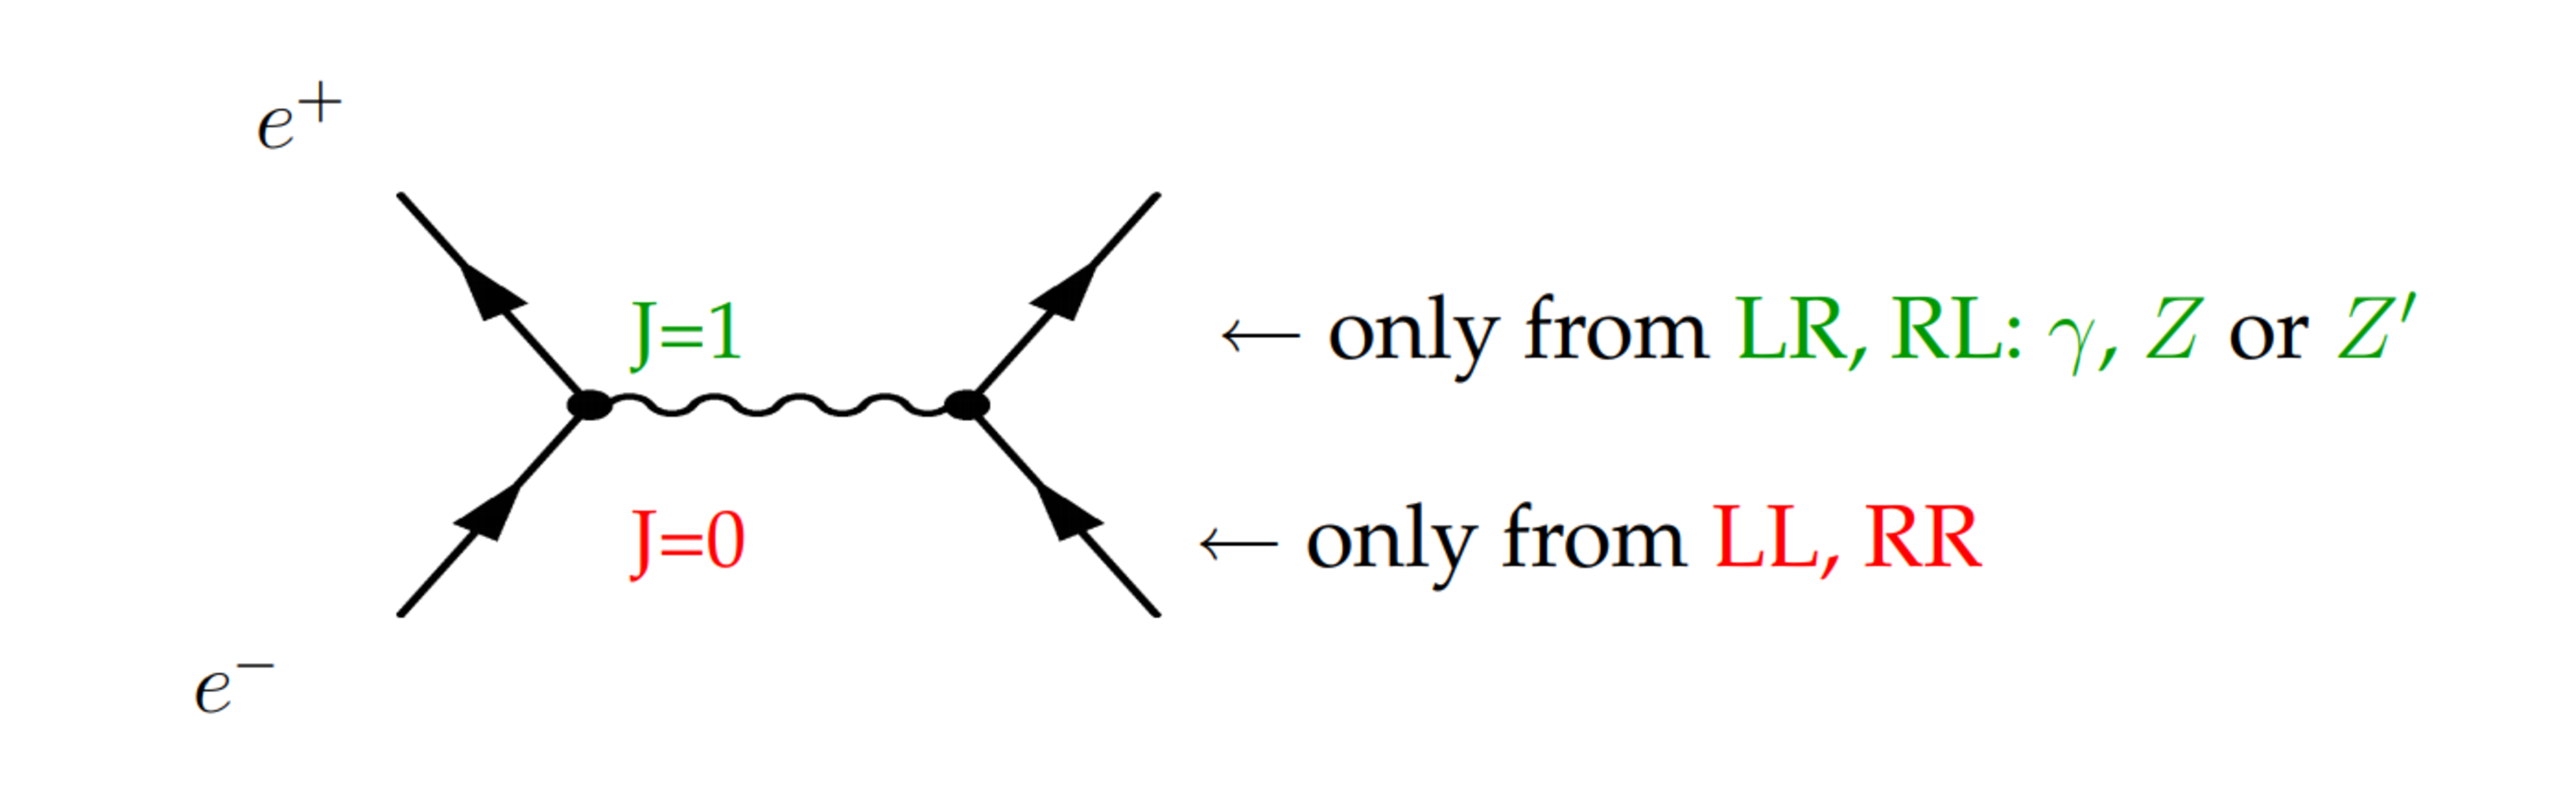
\includegraphics[width=0.49\textwidth]{helicity1.pdf}
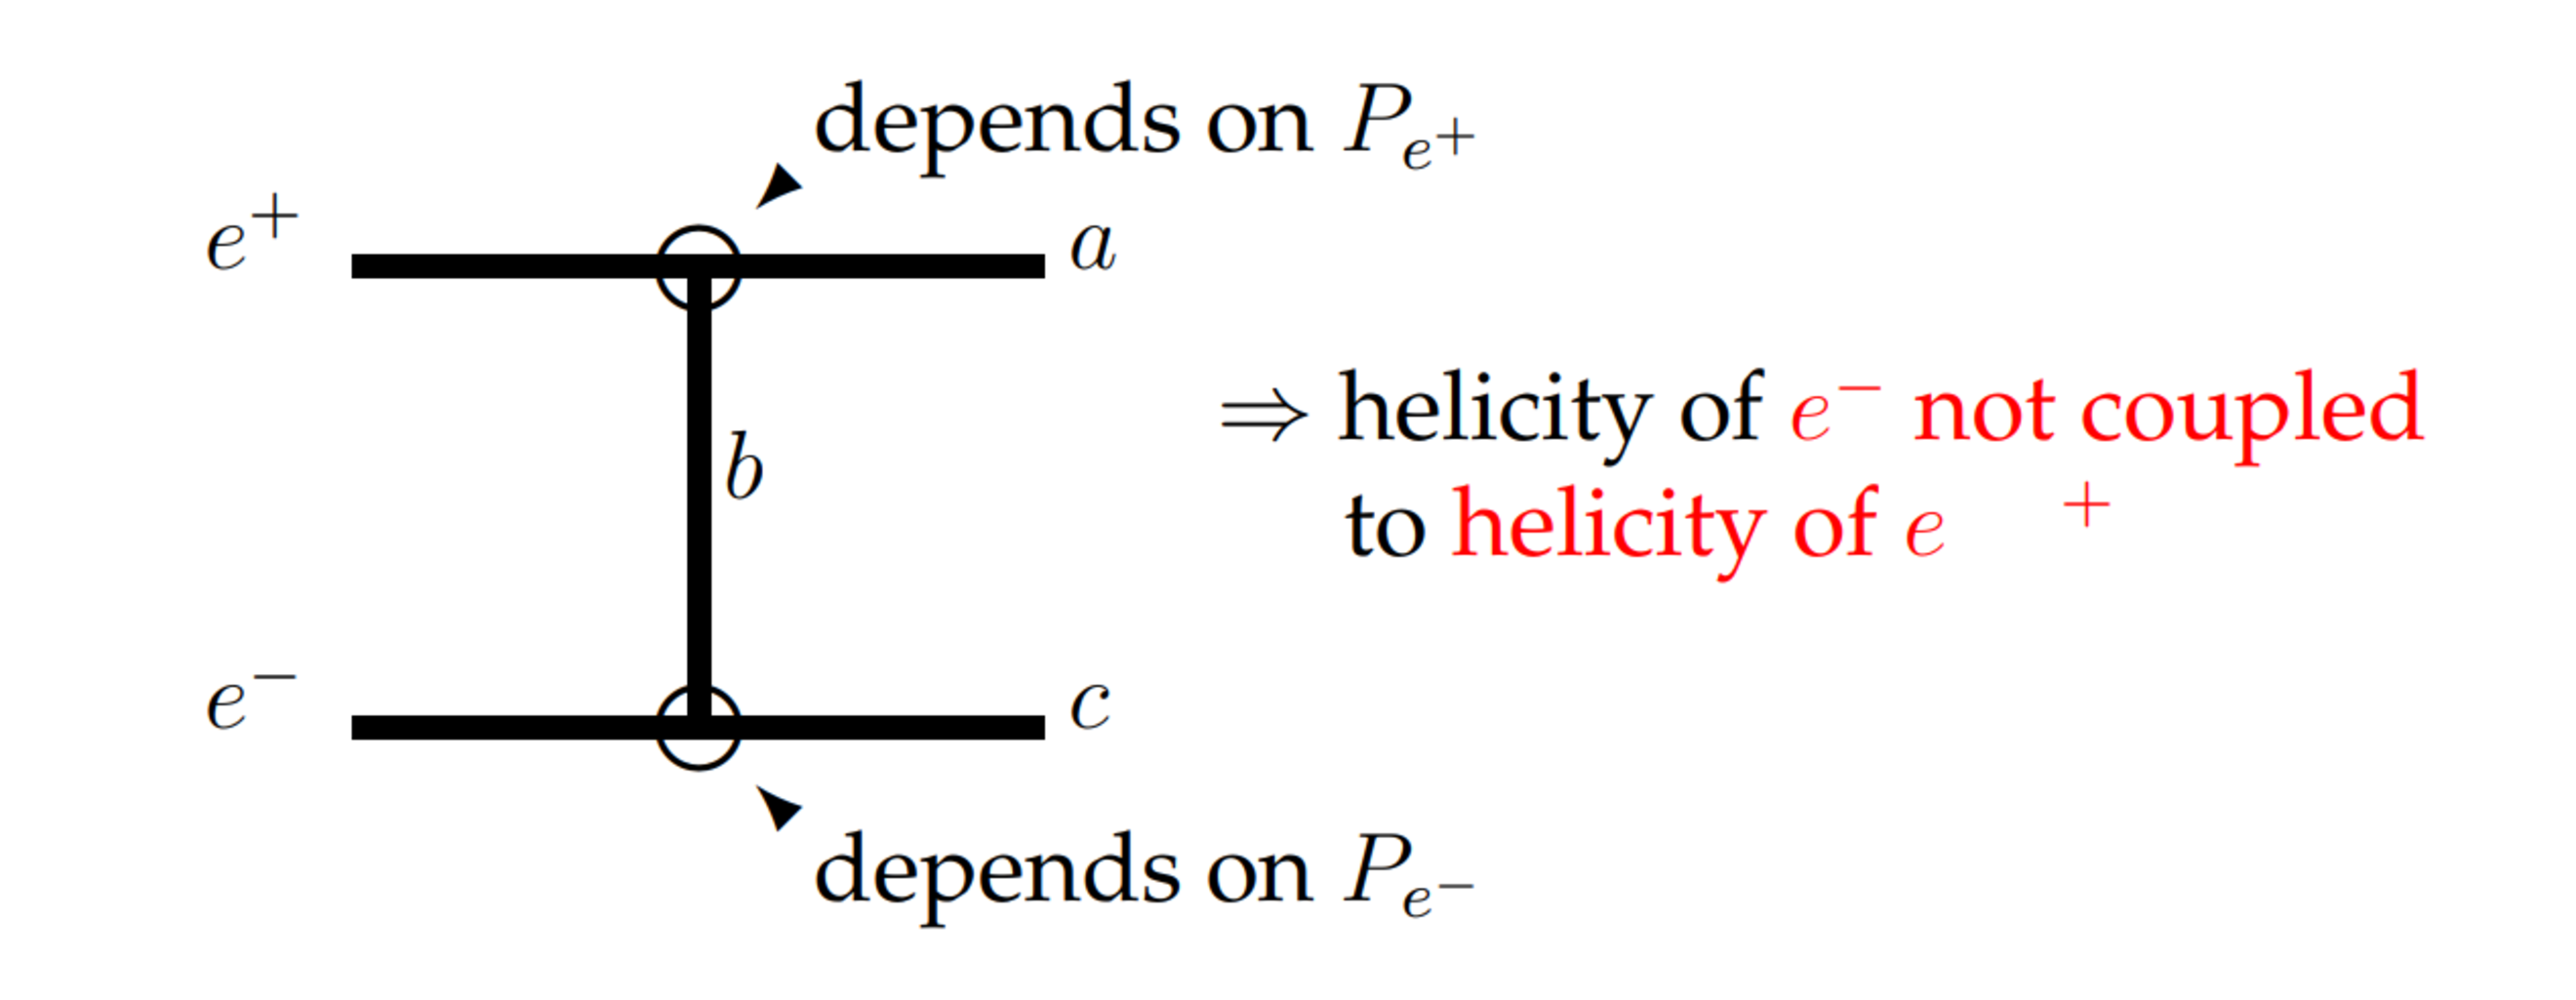
\includegraphics[width=0.49\textwidth]{helicity2.pdf}
\caption{Possible spin configurations in the s and t channel. \cite{helicity}}
\end{figure}


--- \textit{Cross-section}\\
The cross-section is an important measurement because it verifies consistency with the underlying standard model predictions for the rate at which a process occurs. This measurement is doubly important for the WW process because it implicitly provides a in situ measurement of the beam polarizations. By definition, the cross-section is a cross-sectional area and represents the probability of an interaction. The total number of events $N$ observed for a process is given by $ N= \sigma L$ the cross-section is denoted by $\sigma$ and $L$ is the integrated luminosity which is a measure of the total number of collisions. In a physics analysis the desired process(signal) is accompanied other processes(background) that can unfortunately be nearly indistinguishable from the signal events. Topologocial or kinematic cuts are applied to each event to minimize the contamination of background events that enter the signal region when trying to count the number of signal events. This reduces the number of observed events $N$ by the number of events lost to the event selection cuts. Thus the number of events observed is then 
\begin{equation}
N = \sigma  L  \epsilon
\end{equation}
where $\epsilon$ is the efficiency of the signal selection in Monte Carlo simulation. The signal efficiency is defined as:
 \begin{equation}
\epsilon = \frac{\text{The number of signal events that pass selection}}{ \text{The total number of signal events that can be selected}}
\end{equation} 
One thing to note is that for a specific process the cross-section includes contributions from all Feynman diagrams that have the same initial and final state particles. This includes diagrams that are essentially not ``signal-like" for WW examples of these contribution diagrams are given in Figure \ref{fig:offshell}.

\begin{figure}
\begin{fmffile}{feyngraph}
\parbox{100pt}{
\begin{fmfgraph*}(85,75)
\fmflabel{\sm$e^+ $}{v 16}
\fmf{fermion}{v 20,v 16}
\fmflabel{\sm$e^+ $}{v  4}
\fmf{fermion}{v  4,v 20}
\fmf{boson,lab=\sm\cyan$\gamma$}{v 21,v 20}
\fmflabel{\sm$\bar{u} $}{v  1}
\fmf{fermion}{v  1,v 21}
\fmf{fermion,lab=\sm\cyan$\bar{u}$}{v 21,v 23}
\fmflabel{\sm$d\ $}{v  2}
\fmf{fermion}{v 23,v  2}
\fmf{boson,lab=\sm\cyan$W^-$}{v 23,v  0}
\fmflabel{\sm$\nu_e $}{v  8}
\fmf{fermion}{v  0,v  8}
\fmflabel{\sm$e^- $}{v 32}
\fmf{fermion}{v 32,v  0}
\fmfleft{v 16,v 32}
\fmfright{v  4,v  1,v  2,v  8}
\end{fmfgraph*}\\ 
} \quad \parbox{100pt}{
\begin{fmfgraph*}(100,75)
\fmflabel{\sm$e^+ $}{v 16}
\fmf{fermion}{v  0,v 16}
\fmflabel{\sm$\nu_\mu $}{v  8}
\fmf{fermion}{v 11,v  8}
\fmflabel{\sm$\bar{u} $}{v  1}
\fmf{fermion}{v  1,v  3}
\fmflabel{\sm$d $}{v  2}
\fmf{fermion}{v  3,v  2}
\fmf{boson,lab=\sm\blue$W^-$}{v  3,v 11}
\fmf{fermion}{v 15,v 11}
\fmflabel{\sm$\mu^+$}{v  4}
\fmf{fermion}{v  4,v 15}
\fmf{boson,lab=\sm\blue$Z$}{v  0,v 15}
\fmflabel{\sm$e^- $}{v 32}
\fmf{fermion}{v 32,v  0}
\fmfleft{v 16,v 32}
\fmfright{v  8,v  1,v  2,v  4}
\end{fmfgraph*}\\
}
\end{fmffile}
\caption{Non signal-like contributions to the WW cross-section, such that, a pair of final state particles are not constrained to the W mass distribution. }
\label{fig:offshell}
\end{figure}






%------------------------------------------------------------


%------------------------------------------------------------

\section{The ILC and ILD}
\label{sec:ILC_detector}
\subsection{Accelerator Description}
\label{ilc}


The search for new physics drives collider energies higher and higher. The current most powerful operating collider is the Large Hadron Collider(LHC) at CERN with a center of mass energy of 13 TeV. The LHC has a very busy environment with significantly more pile up from many proton-proton collisions than in an electron-positron collider. The proton is also a composite particle, and when the components of the proton collide, the type and the energy of the interaction between them is unknown. These features create a significant challenge discovering new physics as well as producing precision physics measurements. The next frontier in high energy physics is through electron and positron collisions. These types of collisions are amenable to precision measurements because the process has a well defined intitial state with less pile-up as well as no excessive backgrounds from $qq$ collisions. The last major electron-positron collider was LEP, reaching center of mass energies of around 200 GeV which was replaced by the LHC in 2001.  The ILC, featured in Figure \ref{fig:ilc}, is the next proposed future linear collider which would harness center of mass energies from 200 GeV up to a possible 1 TeV upgrade.  The proposed design was originally to start at 500 GeV center of mass energy along a 30 km linear accelerator(linac). Prohibitive costs have pushed the starting center of mass energy to 250 GeV  with a 20 km linac with possible 500 GeV and 1 TeV upgrades as well as luminosity upgrades.  The starting instantaneous luminosity planned to be achieved is $1.35 \times 10^{34} \, \, \text{cm}^{−2}\text{s}^{−1}$, leading to a integrated luminosity of $2 \, \, \text{ab}^{-1}$ after a decade. The acclerator will have tunable beams that can be polarised to LR,RL,RR,LL.\cite{currdetector} A detailed description of the accelerator design can be found in the Technical Design Report \cite{tdraccel}.

\begin{figure}
\label{fig:ilc}
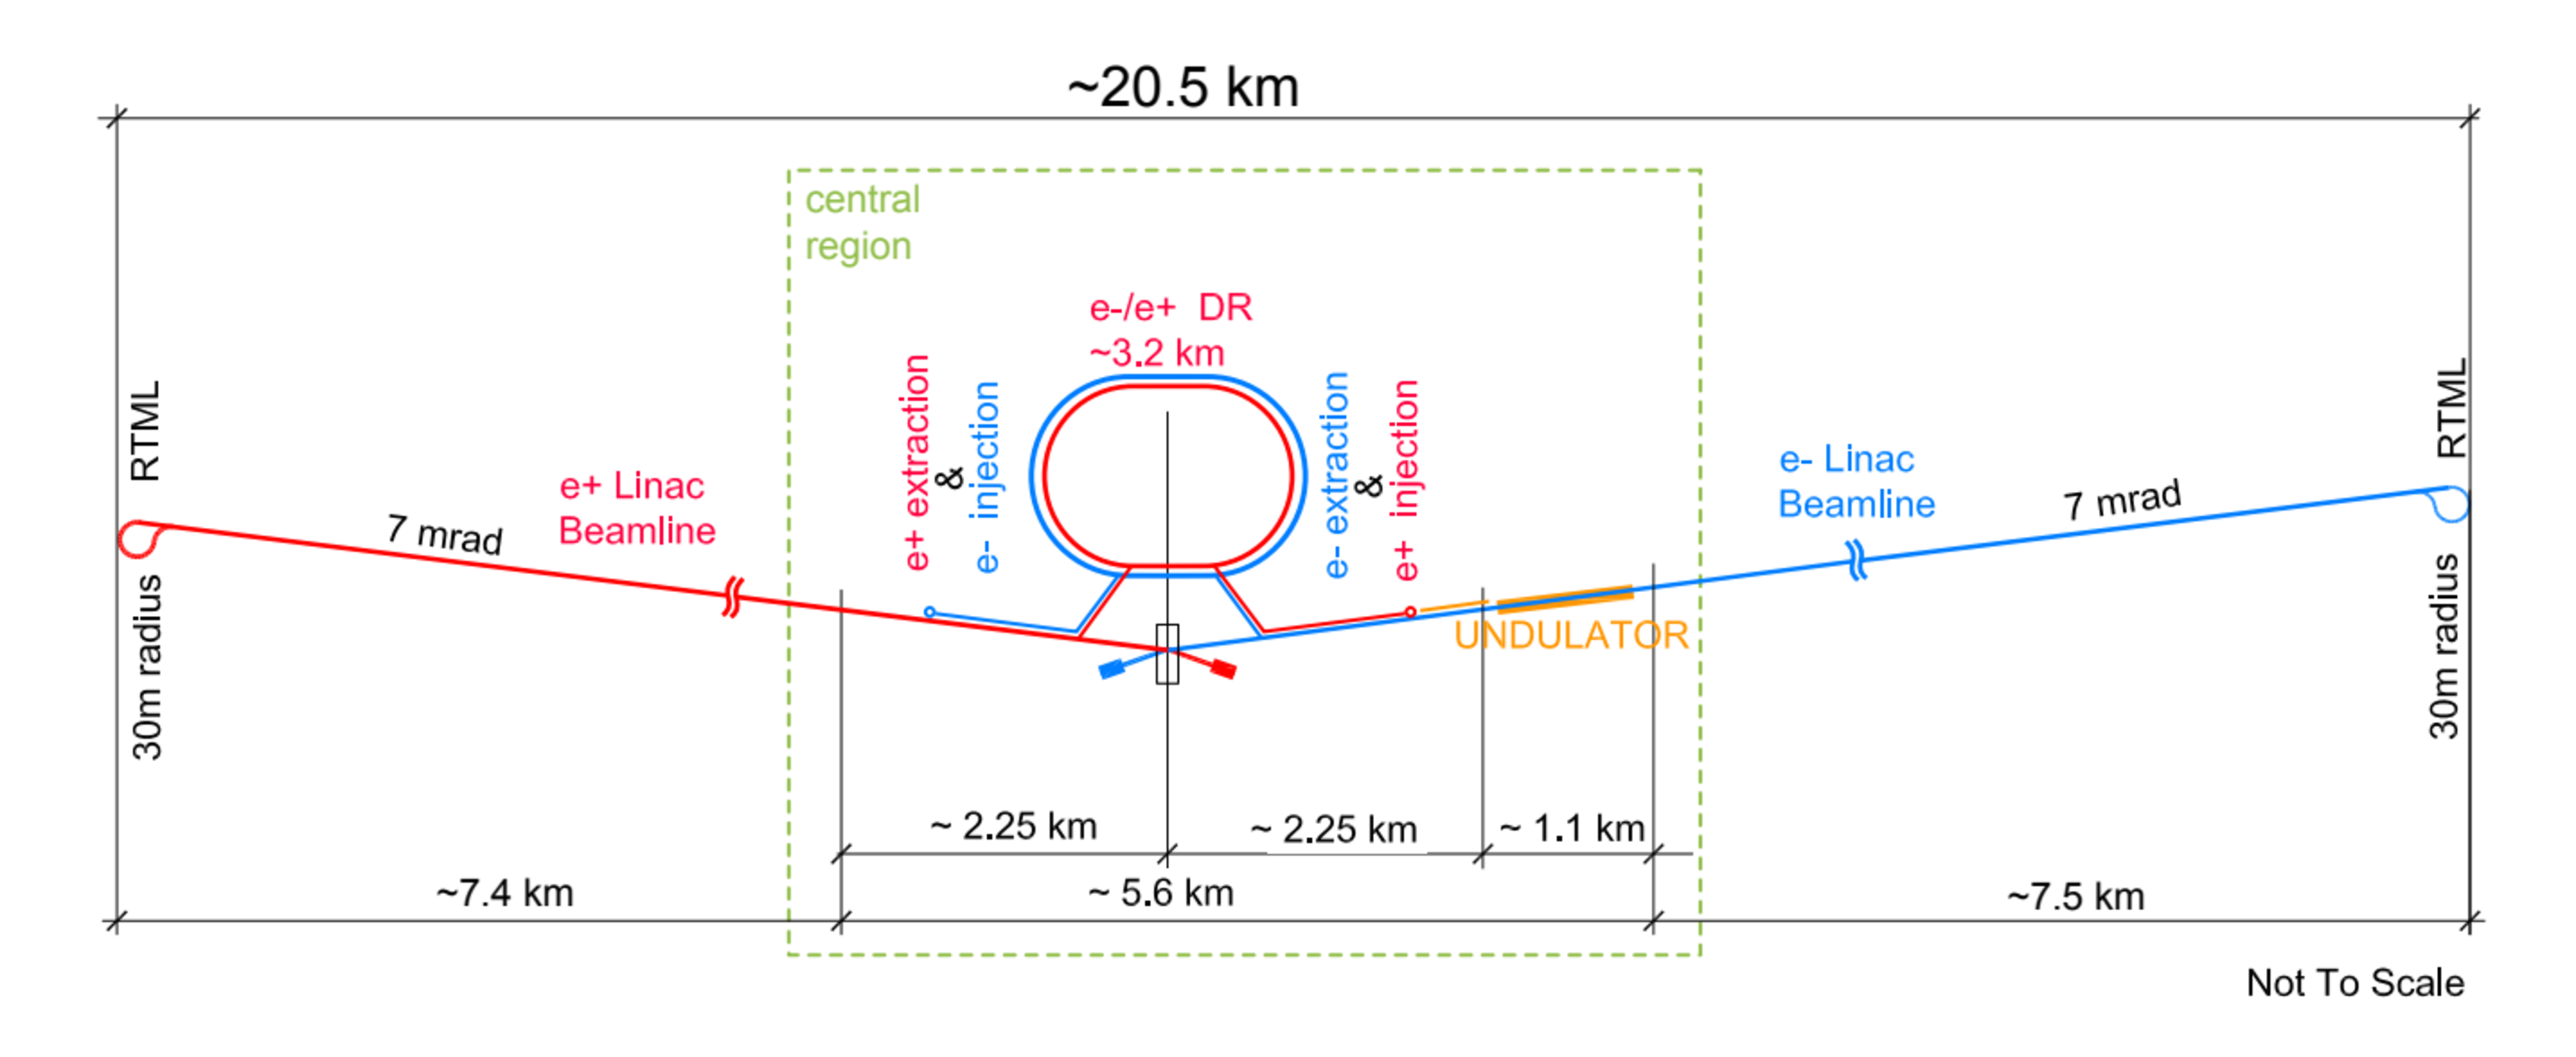
\includegraphics[width=0.9\textwidth]{ilc.pdf}
\caption{Schematic layout of the ILC in the 250 GeV staged configuration \cite{currdetector} }
\end{figure}

\subsection{Detector Description}
\label{ild}

There are two proposed detectors at the ILC which serve the same interaction point on a push-pull mechanism. One detector will take data while the other is under maintenance. This allows for continuous collection of data, the opportunity for complimentary detector designs, competition between detector experiments, and cross-checks between experimental results. All with the benefit of lower overall cost since there is only a single interaction point(IP). The two proposed detectors are the International Large Detector(ILD) and the Silicon Detector(SiD). The ILD concept is feautured in Figure \ref{fig:ilddet}. The accelerator's two opposings beams meet in the center of a detector collide, the collision products then travel outward through the detector.  The detector components form a shell around the beam line and each layer has a specific role in detecting types of particles. The detector layers from the innermost to outermost  is first a vertex detector used to identify the origin of an event, the tracker  which measures the momentum of charged particles, an electromagnetic calorimiter(ECAL) which measures the energy deposited by less massive particles and photons, a dense hadronic calorimeter(HCAL) which stops and contains the showers from more massive particles,  a solenoid which produces a magnetic field bending the trajectory of charged particles in order to distringuish charge, and a external muon layer which detects muons. The forward regions also have a collection of calorimeters designed to capture beam particles scattered at small angles. Both detectors optimize reconstruction of particles by the use of the Particle Flow Algorithm(PFA). The PFA is method that that combines algorithms and a highly granular calorimiter to fully resolve individual particles and their energy deposits \cite{pfa}.
The ILD approach to PFA optimization is by making the detector large, thus creating more physical separation between particles making reconstruction easier. The SiD approach is towards cost efficiency with a smaller detector and stronger magnetic field to try and achieve a similar performance. 
The major difference between the two detectors are the tracking mechanisms.  The ILD plans to use a gaseous central tracker with Time Projection Chamber(TPC). This tracking approach provides nearly continuous path information for tracks by providing up to 224 hits per track. SiD plans to use a silicon tracking system similar to the LHC. The design demands for both detectors are as follows: at least $4 \, \, \mu$m spatial resolution in the vertex detector , a momentum resolution $\Delta (1/p) =  2 \time 10^{-5} \, \, \text{GeV}^{-1}$, a jet energy resolution of at least $3\%$, and hermicity specifically to capture and conserve momentum from particles in the forward region benefitting analyses driven by missing energy \cite{currdetector}.

\begin{figure}
\label{fig:ilddet}
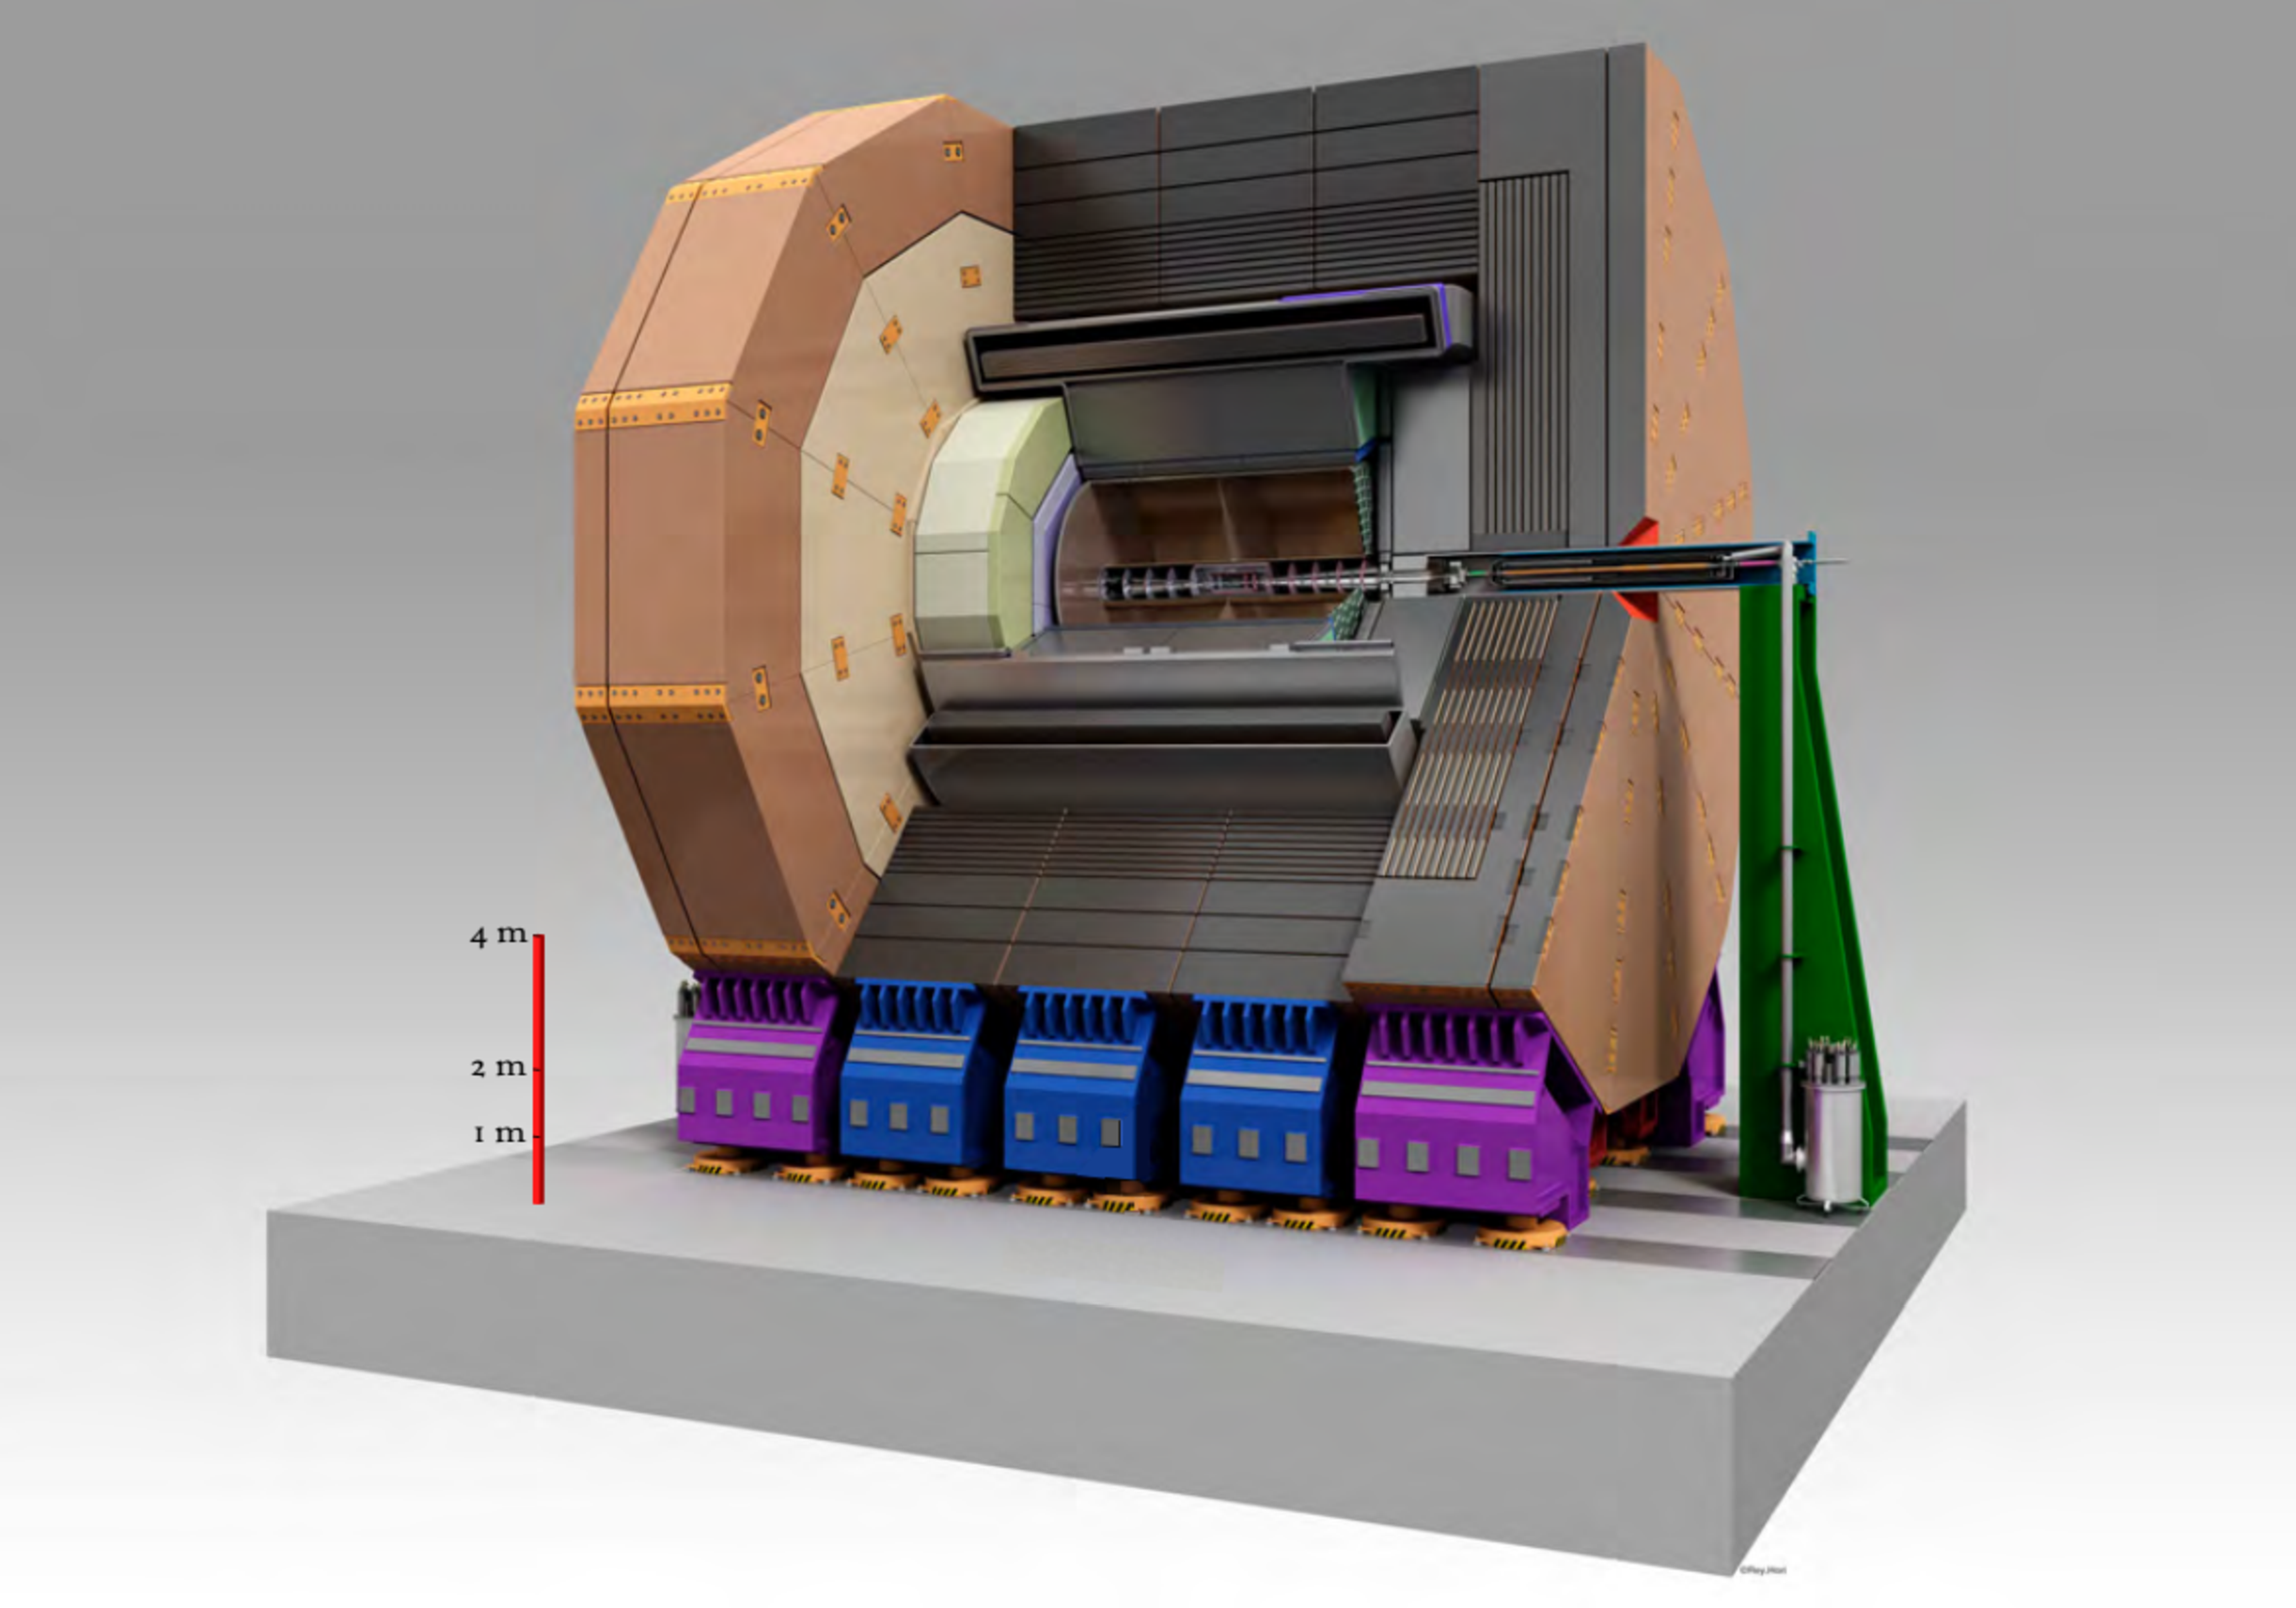
\includegraphics[width=0.49\textwidth]{ild3d.pdf}
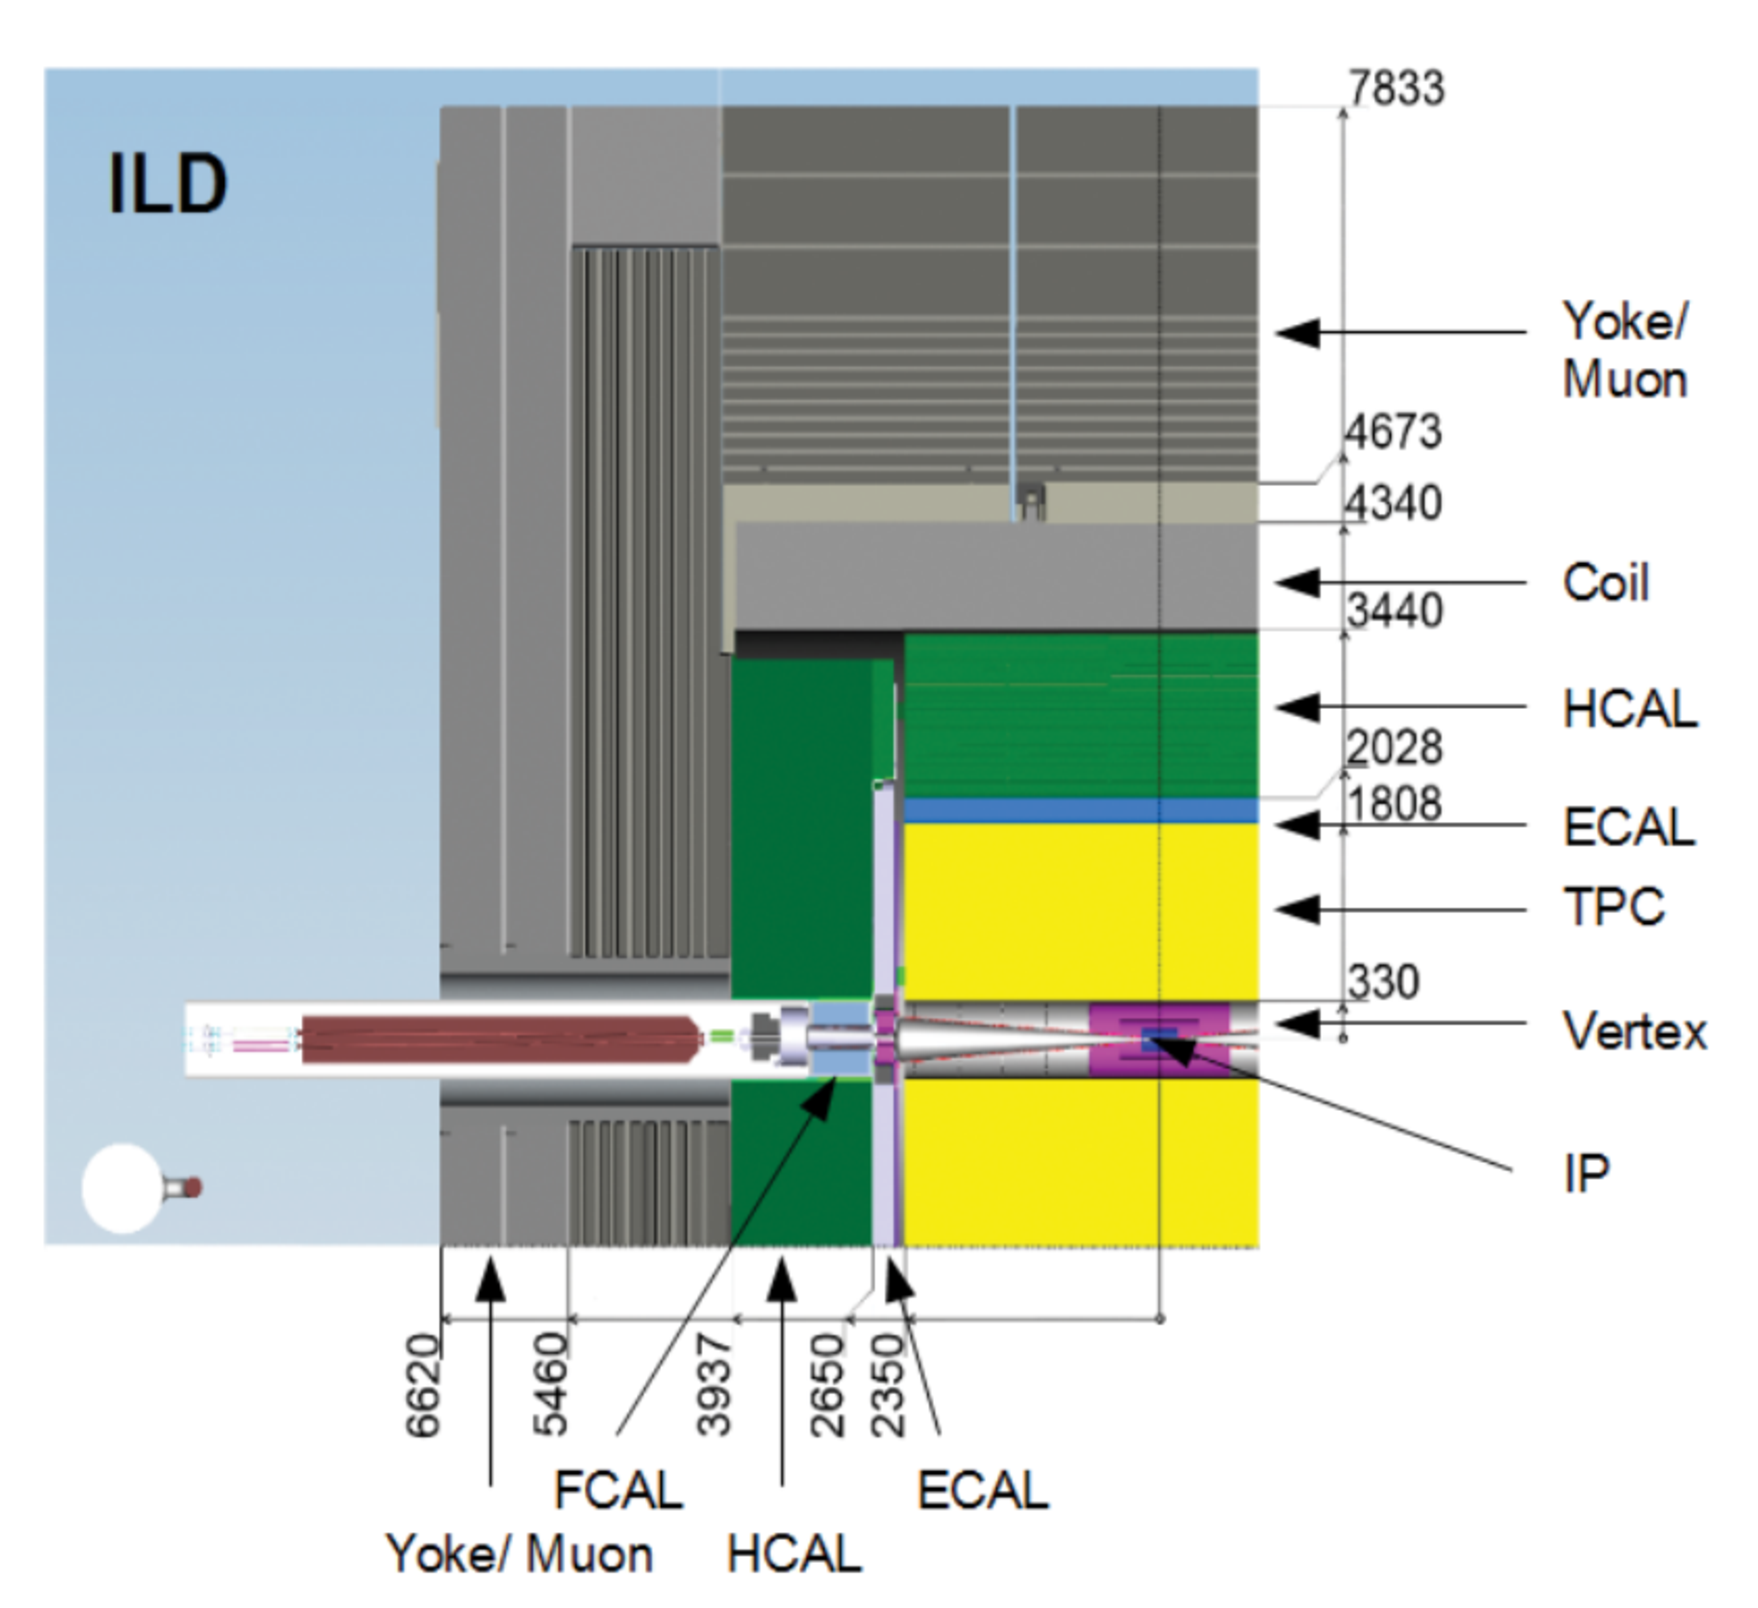
\includegraphics[width=0.49\textwidth]{ildxsec.pdf}
\caption{The ILD concept(Left). Quadrant slice of the ILD and components, dimensions in mm (Right) \cite{tdrdet}.}
\end{figure}
\subsection{Software Packages}
\label{ilcsoft}

The software ecosystem for the ILC is contained under iLCSoft \cite{ilcsoft} which is comprised of reconstruction tools that rely on the event data model LCIO\cite{lcio}, full simulation samples that are generated are based on detector descriptions in DD4HEP \cite{dd4hep}, and physics samples centrally produced with Whizard \cite{ whizard}.




%------------------------------------------------------------

\section{Measurement of the W mass and Cross-section}
\label{Current_Work} 
\subsection{Analysis Overview}
\label{subsec:ana_overview}
The analysis relies on Monte Carlo events that are fully simulated using the ILD detector model \url{ ILD_l5_o1_v02 } with iLCSoft version v02-00-02 and includes a complete standard model background for final states with 2,4, and 6 fermions as well standard model Higgs production.  A center of mass energy of 500 GeV and longitudinally-polarized beams in various operating scenarios are considered. The Monte Carlo events are generated for $100\%$ polarized beams, that is, either all left or right handed. Events are weighted in order to obtain realistic cases of partial polarizations for possible running scenarios which are shown in Table \ref{tab:beamscenario}.

\begin{table}
\label{tab:beamscenario}
\caption{Possible running configurations with partial beam polarizations ($P_{e^-},P_{e^+}$) and integrated luminiosity \cite{ilcop} }
\begin{tabular}{|c|c|c|c|c|}
\hline 
Pol. &(-0.8,+0.3) & (+0.8,-0.3) & (-0.8,-0.3) & (+0.8,+0.3) \\ 
\hline 
$\int$ Lum. [fb$^{-1}$] & 1600 & 1600 & 400 & 400 \\ 
\hline 
\end{tabular} 

\end{table}
 The partial polarizations $P_{e^-} \, \, P_{e^+}$  can be represented by the fraction of the beam which is either left or right handed
 \begin{equation}
 \begin{split}
f_R^{e^-} + f_L^{e^-} = 1 \, \, \, \, \, \, f_R^{e^-} = \frac{1}{2}(1 + P_{e^-}) \\
f_R^{e^+} + f_L^{e^+} = 1 \, \, \, \, \, \, f_R^{e^+} = \frac{1}{2}(1 + P_{e^+})
\end{split}
 \end{equation}
where the beam fraction $f$ is denoted with the polarization subscript and respective beam superscript. For a particular scenario like $(P_{e^-}, P_{e^+}) = (-0.8, +0.3)$ the -0.8 represents an electron beam with $90\% $ left handed electrons mixed with $10\% $ right handed electrons and a positron beam with $65\%$ right handed positrons mixed with $35\%$ left handed positrons. The weight $\omega$ for a specific event with a particular initial state helicities is given by (with example partial polarizations (-0.8,+0.3) ):
 \begin{equation}
 \begin{split} 
 \omega_{LR} = f_L^{e^-}f_R^{e^+} = 0.9 \times 0.65 = 0.585 \\
 \omega_{RL} = f_R^{e^-}f_L^{e^+} = 0.1 \times 0.35 = 0.035 \\
 \omega_{LL} = f_L^{e^-}f_L^{e^+} = 0.9 \times 0.35 = 0.315 \\
 \omega_{LR} = f_R^{e^-}f_R^{e^+} = 0.1 \times 0.65 = 0.065 
 \end{split}
 \end{equation} 

The analysis workflow for semileptonic WW has three distinct stages, the lepton identification and selection, pile-up rejection in the hadronic system, and event selection against against full standard model backgrounds. The analysis is performed with the all four running scenarios with cuts optimized for the dominant WW production mode (-0.8,+0.3). 


\subsection{Lepton Identification}
\label{subsec:Lepton_ID}
The approach towards the identification of leptons relies on treating leptons universally. The easiest lepton to identify is the muon, which produces a single track along with hits in the muon detector. The electron also produces a track in the TPC but is often accompanied by photons via bremsstrahlung radiation. The tau is the most difficult lepton to identify due to its decay into multiple charged and neutral particles. To accommodate all types lepton signatures a cone based approach is used to either capture single tracks or collimated jets with low track multiplicity. The lepton finding cone consists consists of two major structures, a search cone containing the particles that belong to the lepton candidate and an isolation cone whose purpose is to reject a lepton candidate if the search cone is not well-isolated from other particles. The acceptance criteria for cone consists of these parameters:
\begin{itemize}
\item Search cone angle $\alpha$ - The opening (half) angle of the search cone for the lepton jet [rad]
\item Isolation cone angle $\beta$ - The outer isolation cone angle w.r.t to the search cone [rad]
\item Isolation energy - The total energy allowed within the isolation cone region [GeV]
\item Invariant Mass - The upper limit on the lepton candidate mass [GeV]
\item Track multiplicity - The allowed number of tracks in a lepton candidate
\item Minimum $P_t$ seed - the minimum transverse momentum of a track that seeds a lepton candidate [GeV] 
\end{itemize}
An example of the cone and parameters are shown in Figure \ref{fig:cone}. Additional requirements are imposed on all of the reconstructed Particle Flow Objects(PFOs) in the event in order to suppress pile-up particles being included in the lepton jet.
\begin{itemize}
\item $P_t > 0.2$ GeV
\item $|cos\theta| < 0.99$
\end{itemize}
The formation of a lepton candidate follows three steps (1) candidate construction, (2) candidate merging, and (3) isolation testing.
The first step starts with a list of seed tracks sorted by energy in descending order. The track energy is calculated with respect to an assumed mass that is imposed by the Pandora PFA.  A track that qualifies as a seed track forms a new lepton candidate, any track that falls within the search cone of the lepton candidate is added to the lepton candidate. For each newly added particle the energy and momentum is updated for the lepton candidate. Tracks that have been added to a lepton candidate are removed from the track seed list. Next, the neutral particles that fall inside the search cone are added to the lepton candidate. The neutral particles also reside on a list, and are removed from the list if added to a lepton candidate, enforcing uniqueness for each lepton candidate. Lepton candidates are continually formed until the list of seed tracks exhausted. When there are no more candidates to be created, the candidates are subjected to part of the acceptance criteria: the lepton jet mass is required to be below upper mass limit (2 GeV) and the number of charged tracks within the lepton candidate is non-zero and less than or equal to 4. If a lepton jet violates any acceptance conditions it is deleted. The next step in the process is merging. If two lepton candidates fall within each others search cones, the candidates are merged. If the mass or track multiplicity conditions are violated, both lepton candidates are deleted.  All  candidates that survive merging are subjected to the isolation testing. For each candidate, the sum of energy of all the particles that fall inside the isolation cone is computed. If the total energy inside the isolation cone is greater than the maximum allowed energy inside the isolation cone the lepton candidate is deleted.\\
\quad \quad \\
The universal lepton treatment is not conducive to a 1-size fits all approach to lepton ID due to the abundance of different lepton signatures. To accomodate for variations between leptons signatures, the acceptance criteria for leptons is optimized according to lepton flavor and $\tau$ decay topology. The categories created are:\\

\begin{minipage}[h]{0.48\textwidth}
\centering
\begin{itemize}
\item Prompt $\mu$
\item Prompt $e$
\item $\tau \rightarrow \mu \bar{\nu_{\mu}} \nu_{\tau} $
\item $\tau \rightarrow e \bar{\nu_{e}} \nu_{\tau} $
\item $\tau \rightarrow$ hadrons (1-prong)
\item $\tau \rightarrow$ hadrons (3-prong)
\end{itemize}
\end{minipage}\hfill
\begin{minipage}[h]{0.48\textwidth}
\label{fig:cone}
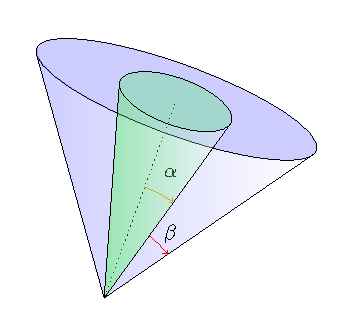
\includegraphics[width=0.6\textwidth]{cone.pdf}
\captionof{figure}{Illustration of possible lepton candidate cone with search cone angle $\alpha$ and isolation cone angle $\beta$. The search cone is shown in green and the isolation cone is the surrounding blue cone.}

\end{minipage}\\

The Prompt categories refer to events which the leptonic W decays directly to either a muon or electron and associated neutrino. The tau categories address the various dominant decay topologies of the tau lepton. For each category, the optimal lepton acceptance criteria is calculated with respect to the events that match the desired topology. The optimal acceptance criteria is the set of parameters that maximally identify lepton candidates that originate from true leptons and minimize the fake lepton candidates that originate from hadronic jets. To find this set of parameters, a scan over a 3D space is performed using the search cone-$\alpha$, isolation cone-$\beta$, and isolation energy-$E_{iso}$. The invariant mass is held at a fixed 2 GeV for simplicity.
Two uncorrelated push-pull parameters are defined to find the optimal working point in the lepton finding space. The first is related to correctly identifying jets originating from true leptons. This is denoted as the efficiency of reconstructing a true lepton $\epsilon_T$. The second optimization parameter is denoted as $P_F$, the probability of a fake lepton jet arising from a single hadronic jet.  
\begin{equation}
\label{eq:et}
\epsilon_T = N_{match}/N_{Stotal}
\end{equation}
\begin{equation}
\begin{split}
\label{eq:pf}
P_F = 1-(1-\epsilon_F)^{\frac{1}{4}} \\
\epsilon_F = N_{fake}/N_{Btotal}
\end{split}
\end{equation}
The true lepton reconstruction efficiency is maximized with the signal sample $WW\rightarrow q\bar{q}\ell\nu$. The denominator represents the total, category specific, number of events which contain three generator visible fermions. The true $q\bar{q}\ell$ fermions are required to fall within the acceptance range $|cos\theta| < 0.99$. $N_{match}$ is the number of signal sample events in which a lepton candidate is reconstructed and can be matched to the true lepton, such that the opening angle between the reconstructed lepton and the true lepton are less than 0.1 radians. The distribution of opening angles is shown if Figure \ref{fig:taupsi}. In the case that a reconstructed lepton is being matched to a true tau, the matching angle formed between the reconstructed lepton and the vector sum of the visible generator components of the tau decay. The visible components of the tau decay consist of the direct decay products whereas photons from final state radiation are excluded. The fake lepton probability $P_f$ is minimized using the background sample $WW\rightarrow q\bar{q}q\bar{q}$ and is a function of the fake lepton reconstruction efficiency $\epsilon_F$. The denominator for fake is also subjected to the same acceptance range $|cos\theta| < 0.99$ for all four fermions. The numerator is the total number of events  that contain at least one reconstructed fake lepton. The fake efficiency can be interpreted as the binomial probability of $r$-successes(lepton reconstructions) in 4 trials(hadronic jets). The probability of a single success in a single trial, $P_F$, can be directly derived from the Binomial p.d.f using the fake efficiency $\epsilon_F$. The optimal parameters $\alpha$, $\beta$, $E_{iso}$ for each lepton category are extracted from max$[(1-P_F)\epsilon_T]$. The results for each category are shown in Table \ref{tab:taufinderopt}. 


\begin{figure}
\centering
    \begin{minipage}{0.48\textwidth}
        \centering
\label{fig:taupsi}
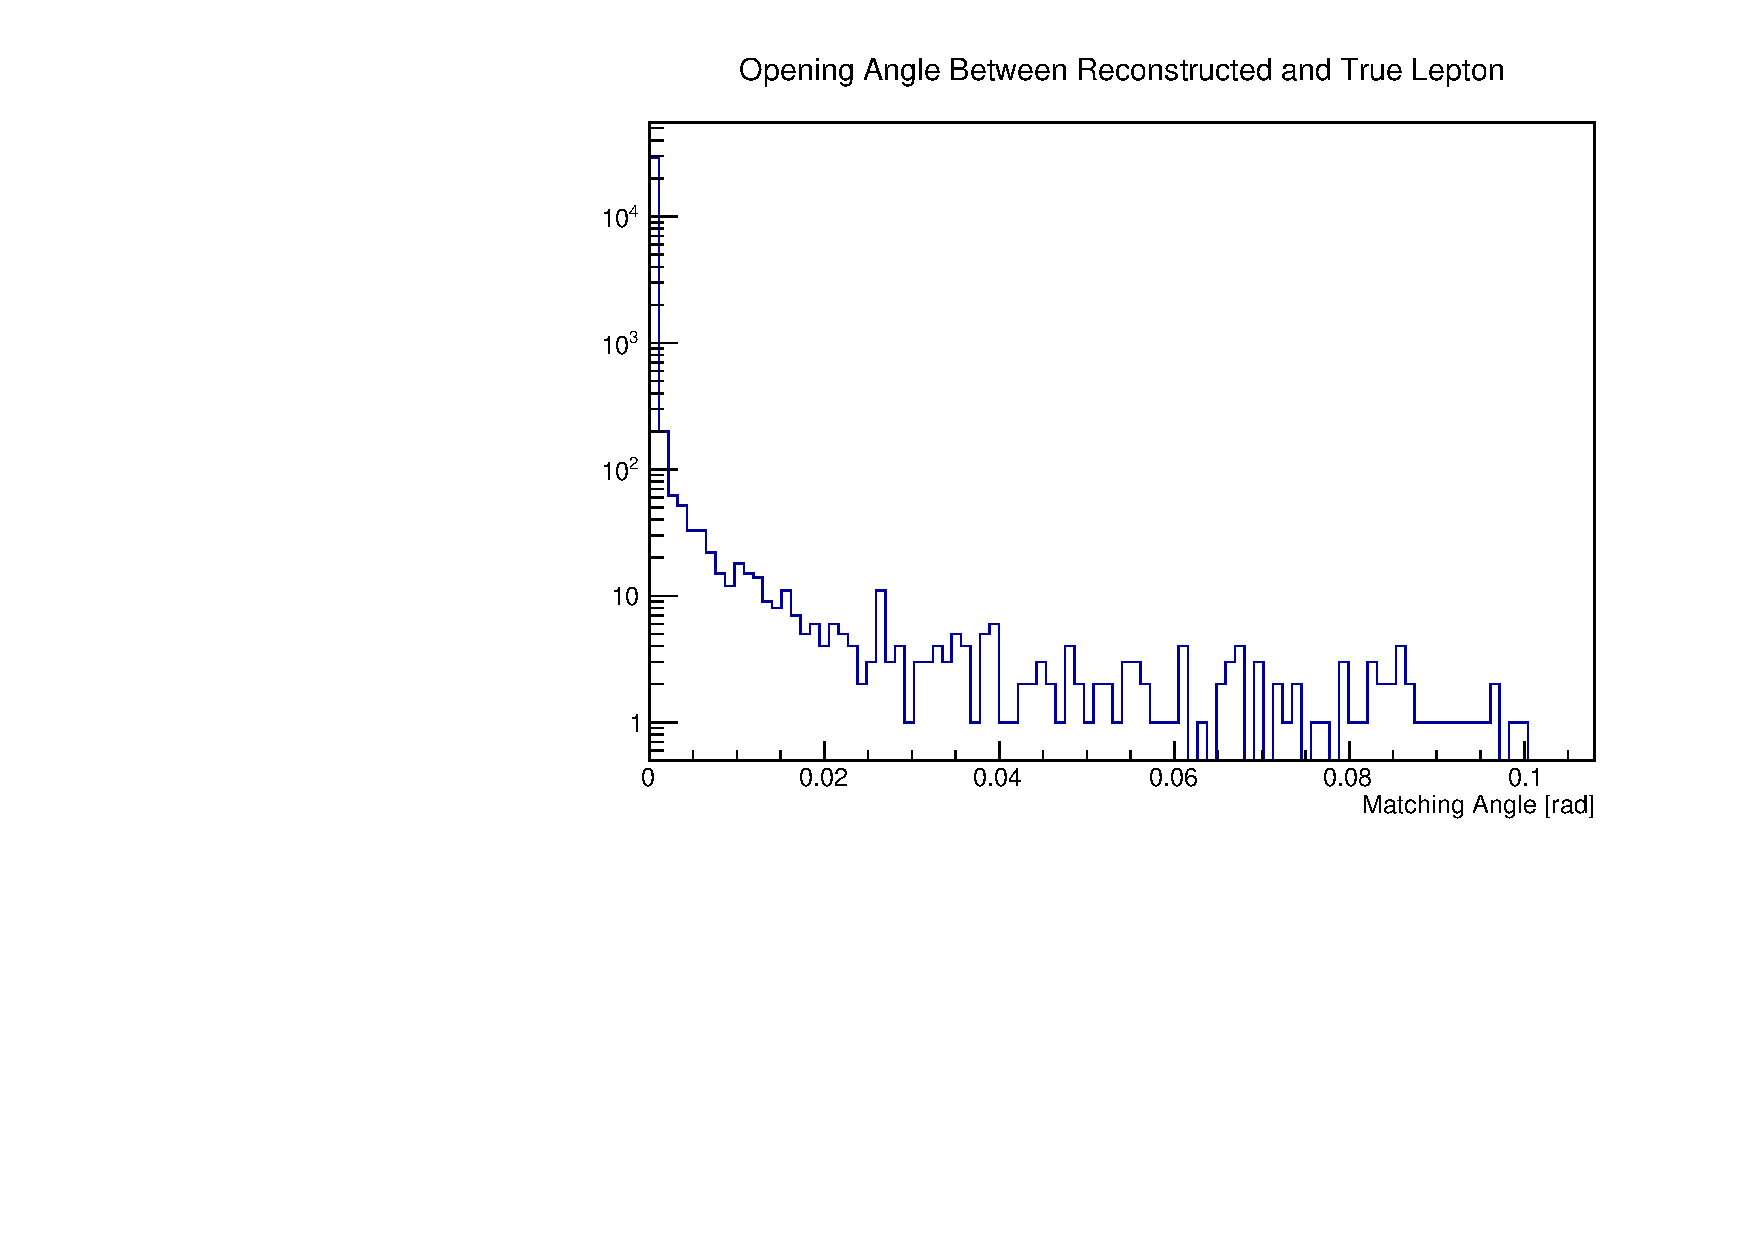
\includegraphics[width=0.9\textwidth]{matchingangle.pdf}
\caption{Distribution of opening angles between the closest reconstructed lepton candidate and the true muon from $WW \rightarrow q \bar{q} \mu \nu_\mu$. $99.4\%$ of events with a muon candidate are matched to truth.} 
\end{minipage}\hfill
    \begin{minipage}{0.48\textwidth}
        \centering
\label{fig:candE}
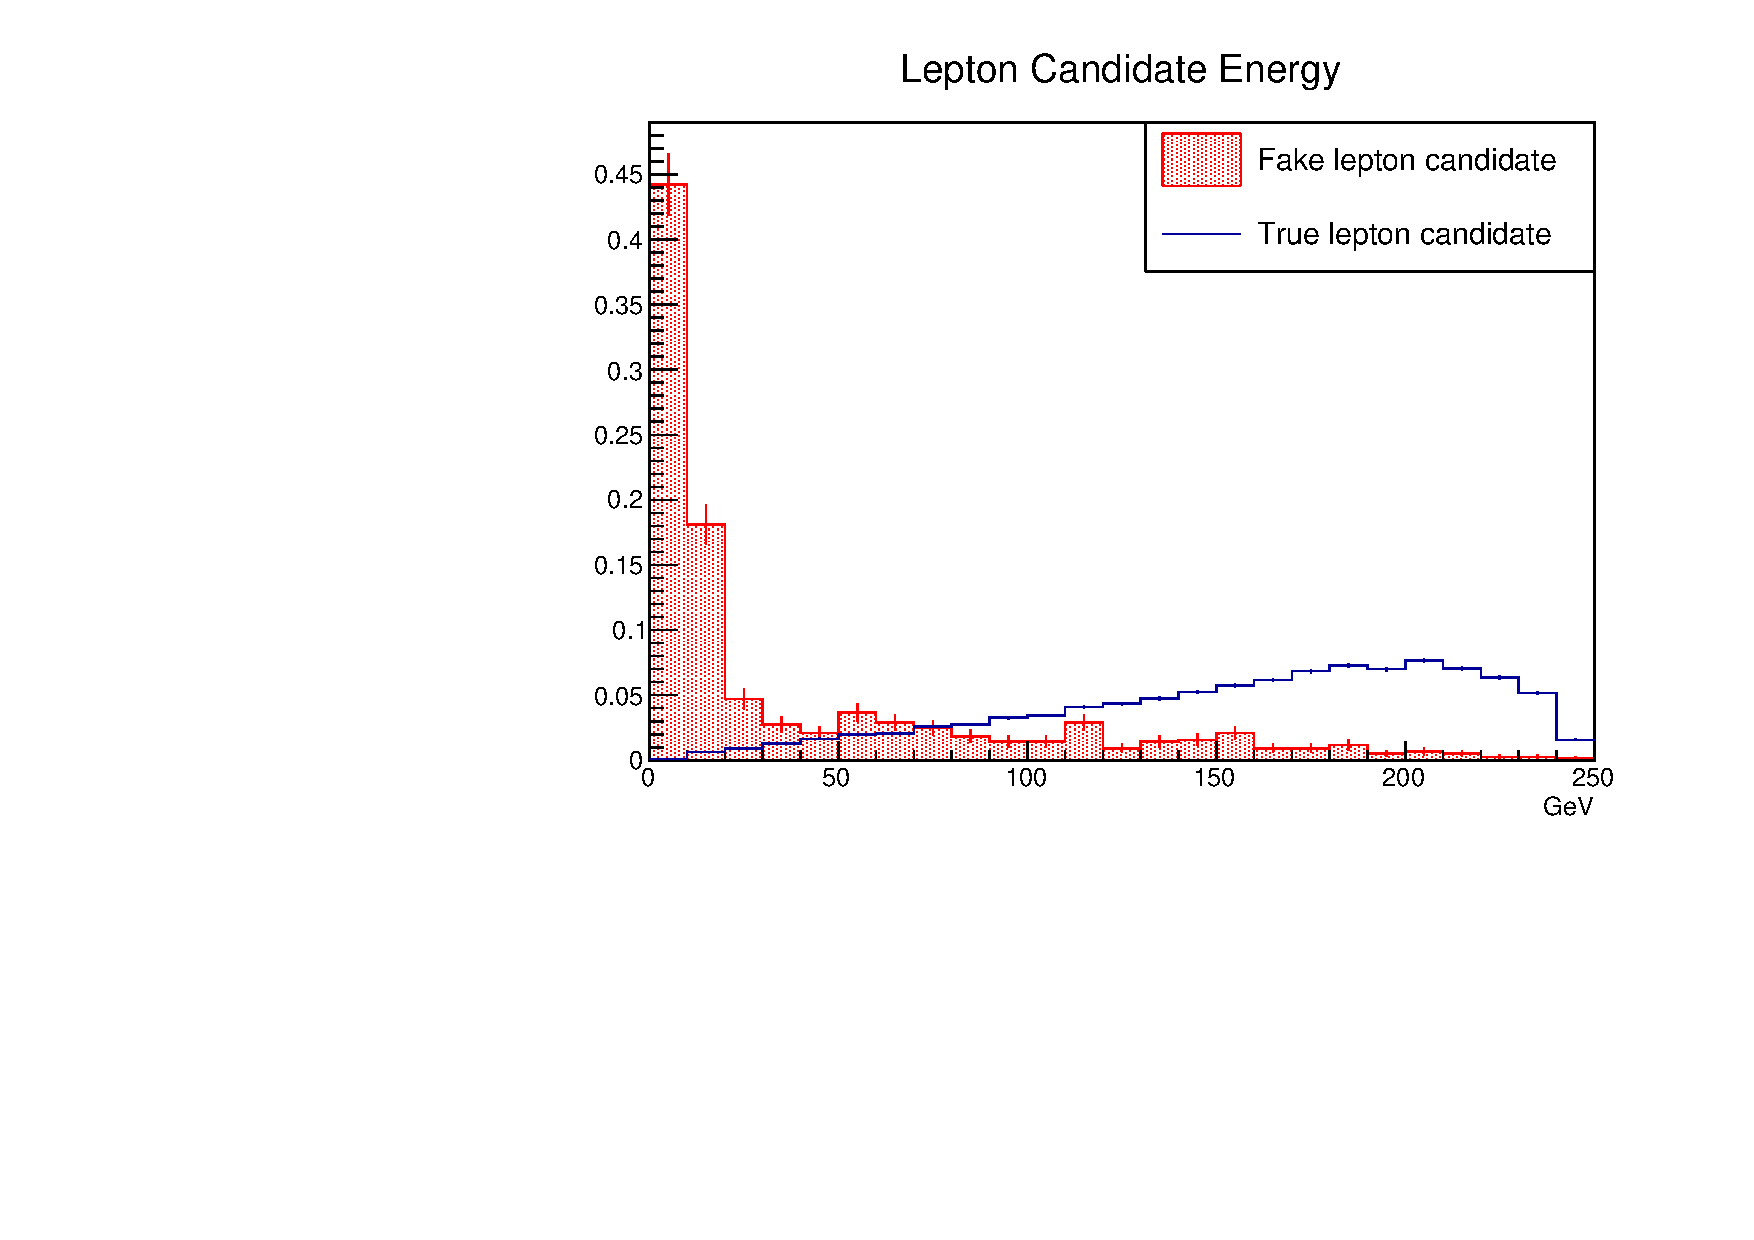
\includegraphics[width=0.9\textwidth]{candEnergy.pdf}
\caption{Energy distribution of lepton candidates matched to truth from $WW \rightarrow q \bar{q} \mu \nu_\mu $ and fake candidates from $ WW \rightarrow q\bar{q} q \bar{q}$ both normalized to unity.}
\end{minipage}
\end{figure}



\begin{table}
\label{tab:taufinderopt}
\begin{tabular}{|p{0.15\textwidth}|p{0.16\textwidth}p{0.16\textwidth}p{0.16\textwidth}p{0.1\textwidth}p{0.1\textwidth}p{0.1\textwidth}|}

\hline 
Channel & $n \, \, \text{Lep} \geq 1$ & $1-P_{F}$ & $\epsilon_T$ & SearchCone [rad] & Iso.Cone [rad] & Iso.E [GeV] \\ 
\hline 
Prompt $\mu$ & $0.955 \pm 0.003$ & $0.974 \pm 0.001$ & $0.949 \pm 0.003$ & 0.03 & 0.15 & 3.0 \\ 

Prompt $e$ & $0.920 \pm 0.003$ & $0.961 \pm 0.001$ & $0.904 \pm 0.003$ & 0.04 & 0.15 & 4.0 \\ 

Inclusive $\tau$ & $0.800 \pm 0.005$ & $0.943 \pm 0.001$ &  $0.770 \pm 0.006$ & 0.07 & 0.15 & 4.5 \\ 


 \hline
$\tau \rightarrow \nu \nu \mu$ & $0.815 \pm 0.012$ & $0.974 \pm 0.001$ & $0.801 \pm 0.013$ & 0.03 & 0.15 & 3.0 \\ 
 
$\tau \rightarrow \nu \nu e$ &  $0.800 \pm 0.012$ & $0.963 \pm 0.001$ &  $0.781 \pm 0.013$ & 0.05 & 0.15 & 3.5 \\ 
 
$\tau$ Had-1p & $0.744 \pm 0.009$ & $0.930 \pm 0.002$ & $0.707 \pm 0.009$ & 0.07 & 0.15 & 4.5 \\ 
 
$\tau$ Had-3p &  $0.756 \pm 0.015$ & $0.930 \pm 0.002$ & $0.710 \pm 0.016$ & 0.07 & 0.15 & 5.5  \\
\hline
\end{tabular} 
\caption{Optimization results using $100 \%$ LR $q\bar{q}\ell \nu$ and $q\bar{q} q\bar{q}$ samples. The $n \, \, \text{Lep} \geq 1$ column pertains to signal samples where at least one lepton candidate was found and is not subjected to the truth matching criteria of 0.1 radians. Results shown are the configurations that maximize $(1-P_F)\epsilon_T$ }
\end{table}

Since only one lepton is expected from signal, a single lepton candidate is selected as the candidate for the event. If multiple lepton jets are reconstructed the lepton candidate with the highest energy is selected as the single candidate for the event. The energy distribution of true and fake leptons is shown in Figure \ref{fig:candE}. If the two highest energy lepton jets are of equal energy then the candidate selected will be the jet with the highest energy original seed track, due to seed track sorting.  Any additional lepton candidates not selected are treated as part of the hadronic system.


\subsection{Pileup mitigation}
\label{subsec:Pileup_mitigation}
\begin{figure}
\label{fig:Epartition}
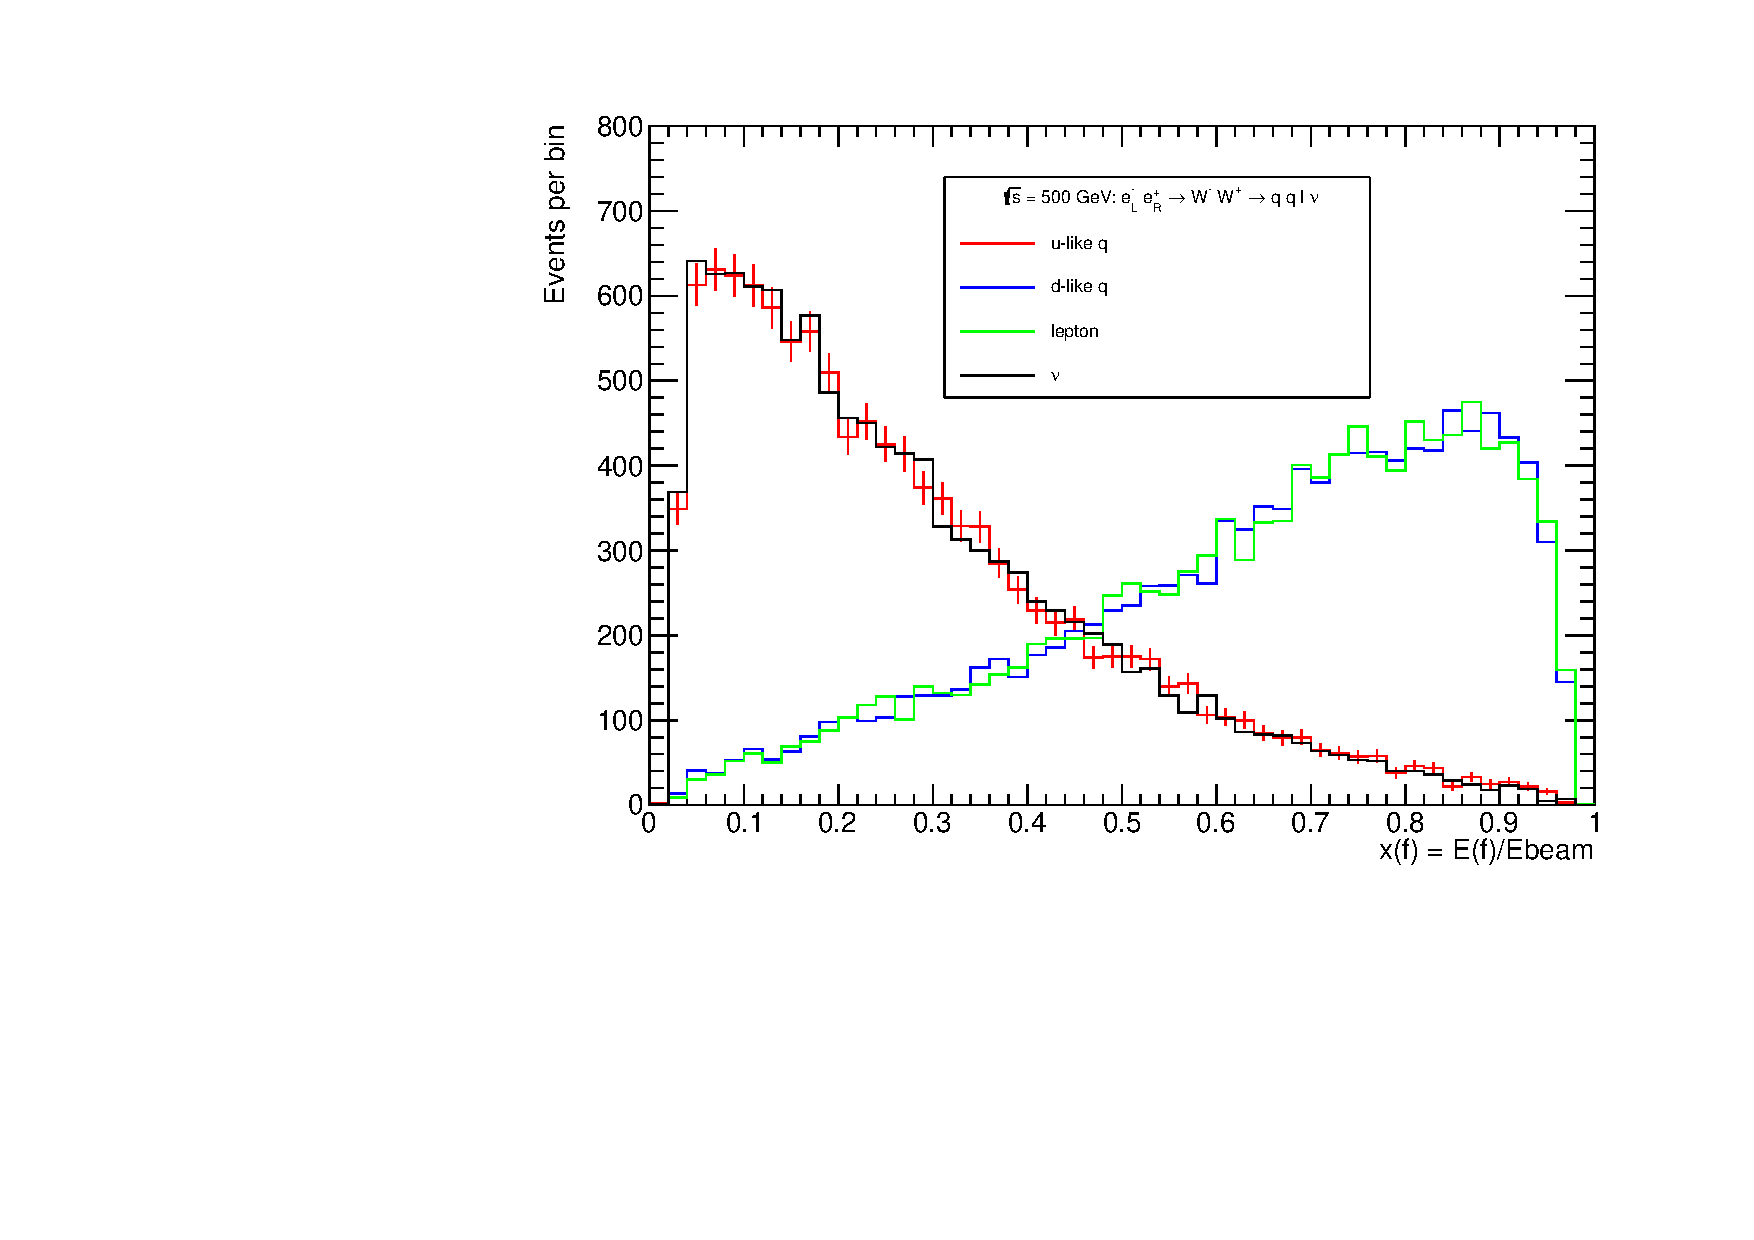
\includegraphics[width=0.48\textwidth]{hxLR.pdf}
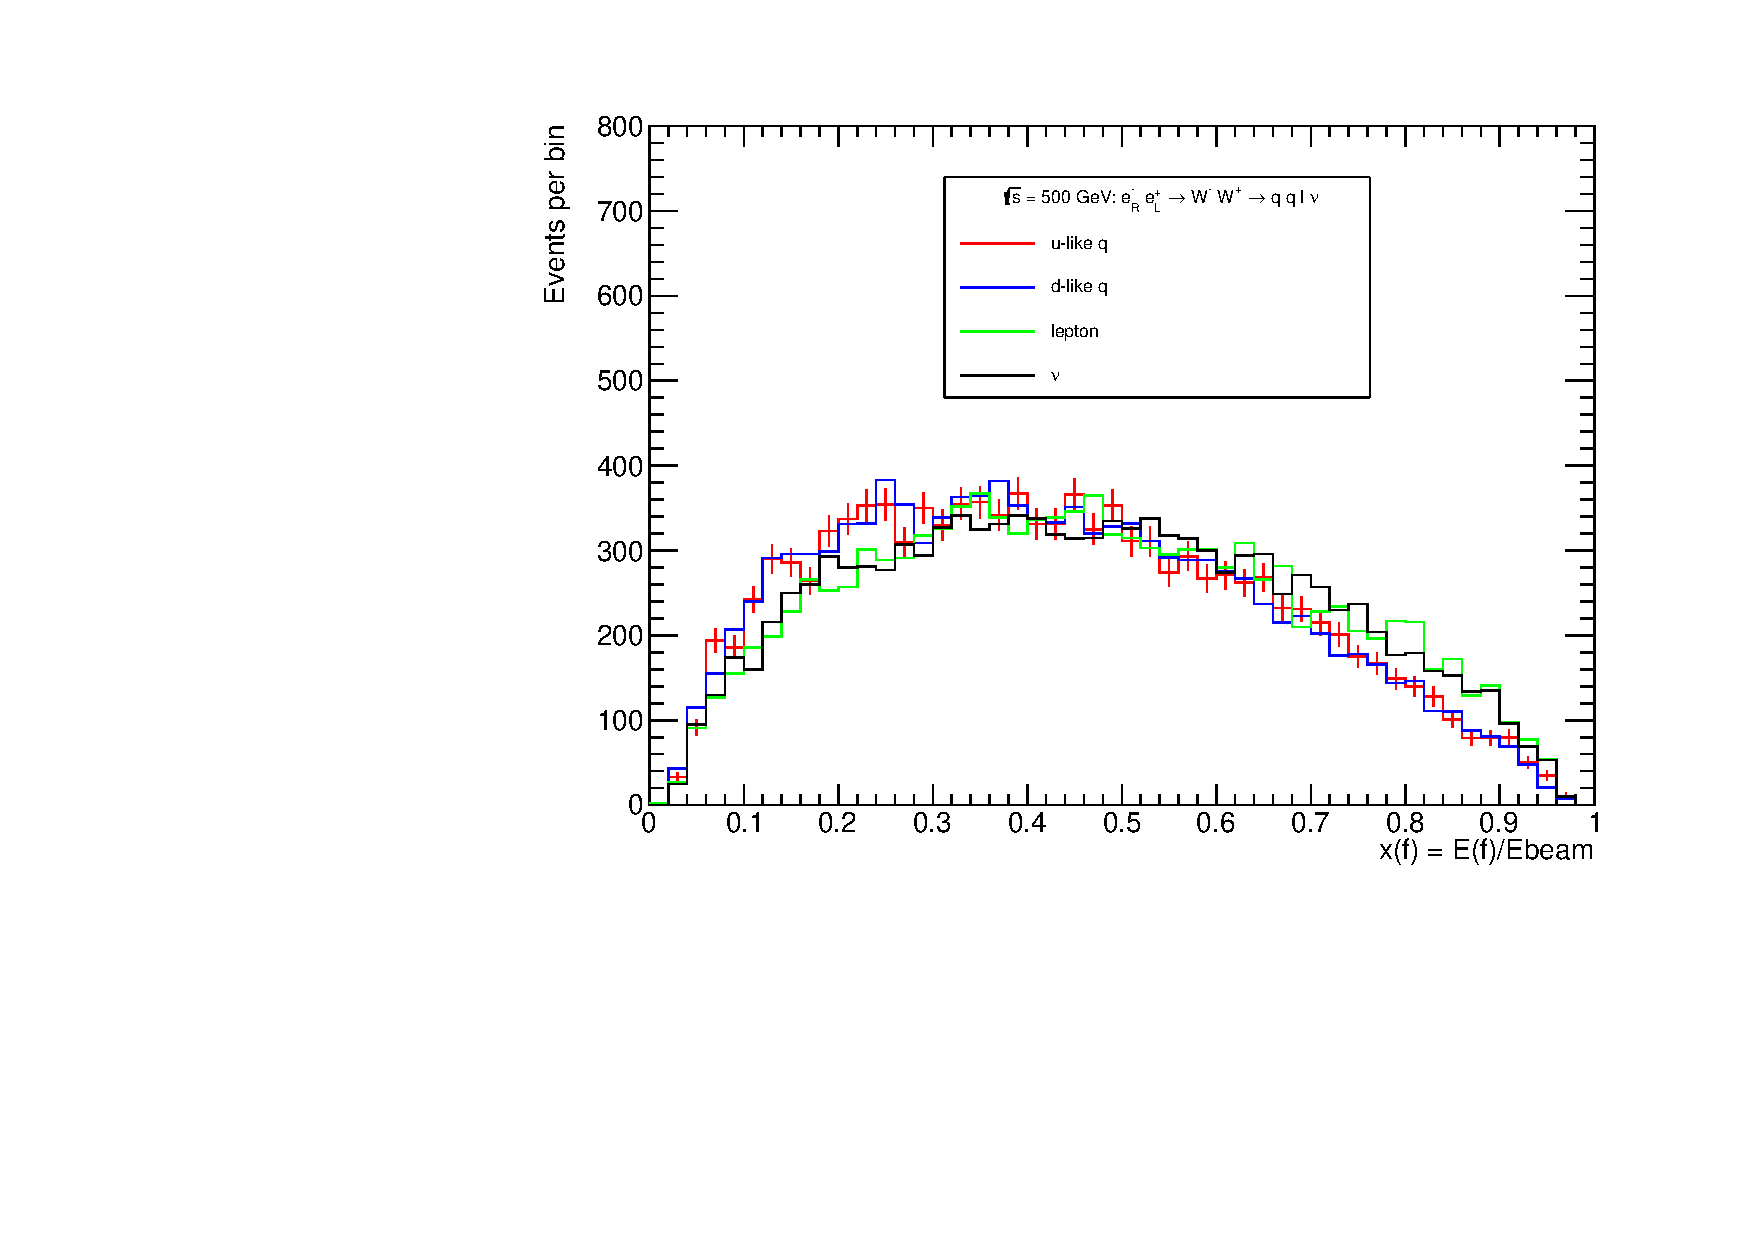
\includegraphics[width=0.48\textwidth]{hxRL.pdf}
\caption{The fractional energy partitioning of the true fermions with $\ell = \mu,\tau$, $100\%$ polarization for the initial state helicities LR(Left) and RL(Right) at center of mass energy 500 GeV. In the LR configuration the charged lepton and down-like quark take the majority of the beam energy. In RL the energy partitioning is even between the four fermions. }
\end{figure}

\begin{figure}

\label{fig:fangles}
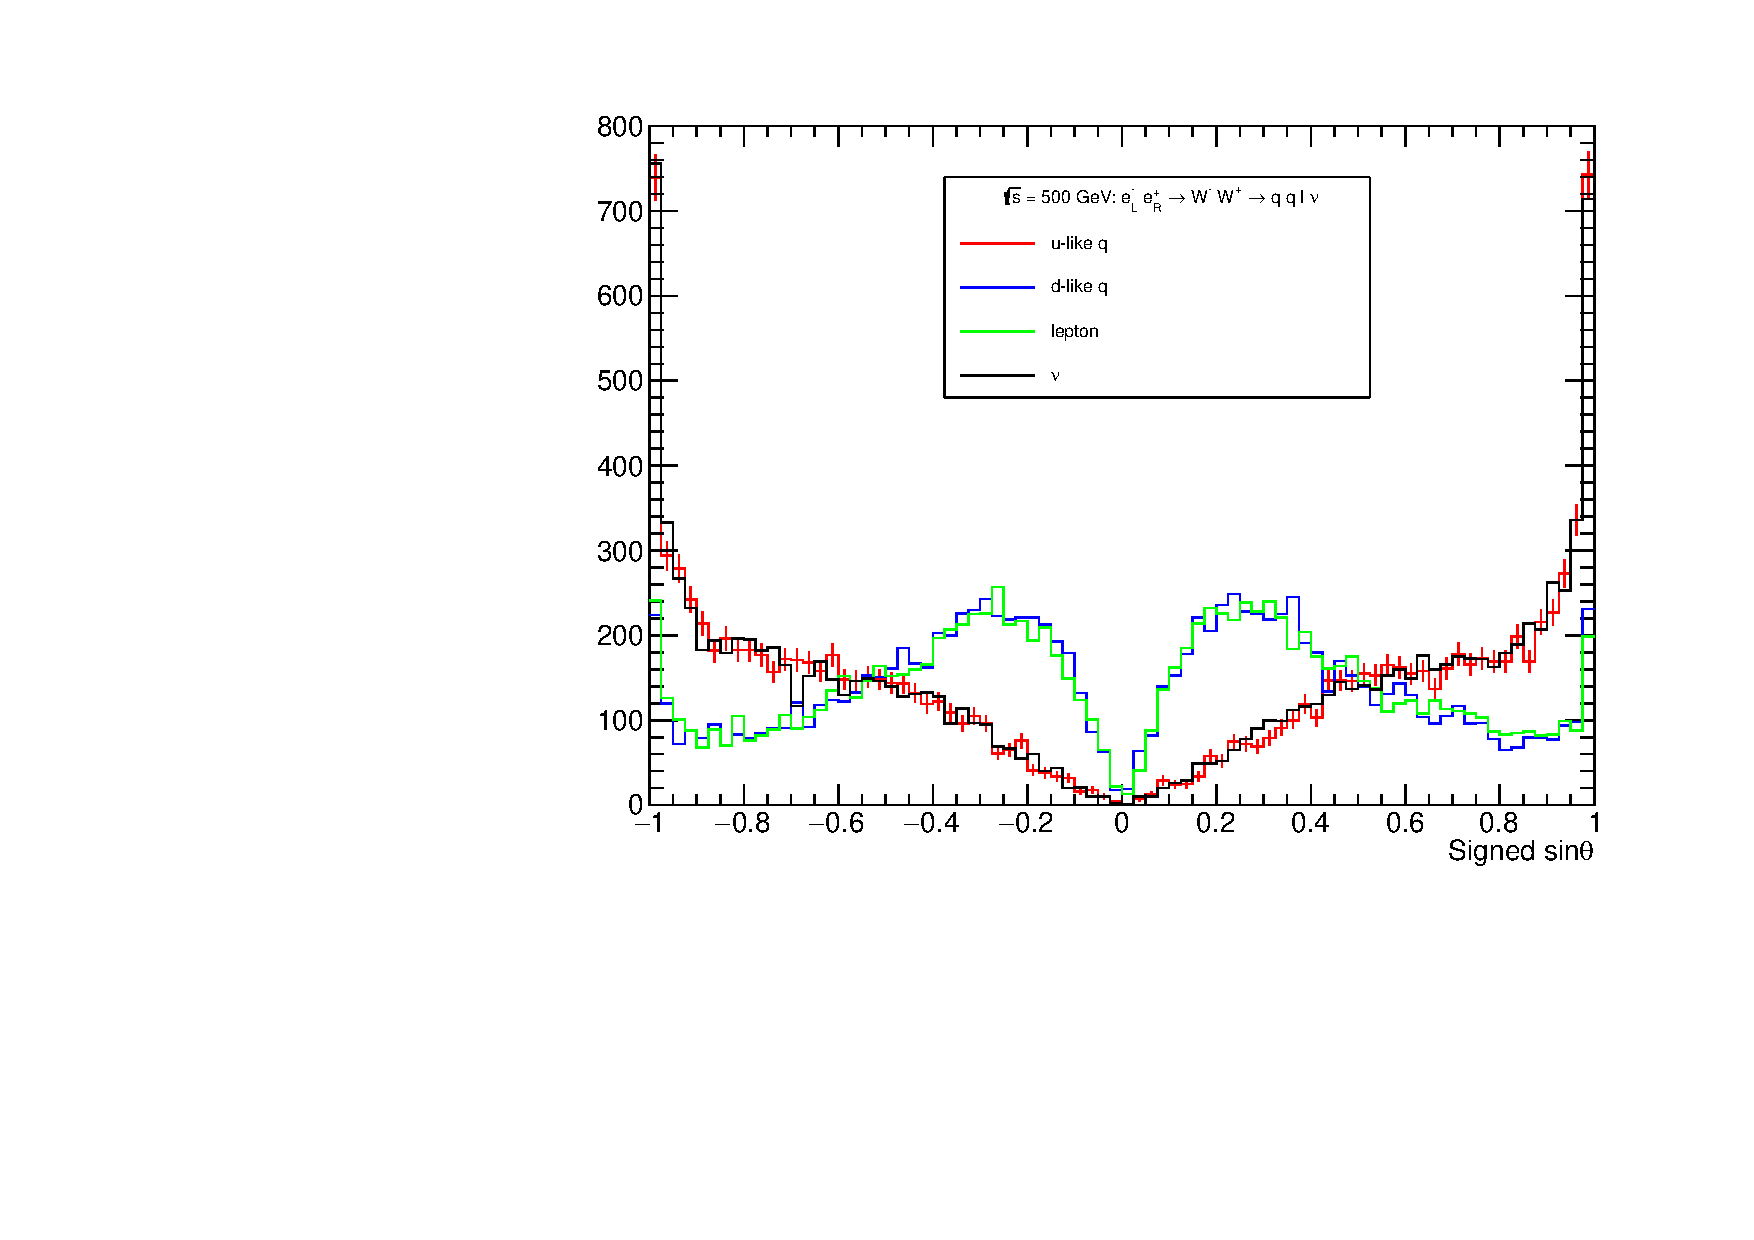
\includegraphics[width=0.48\textwidth]{hsLR.pdf}
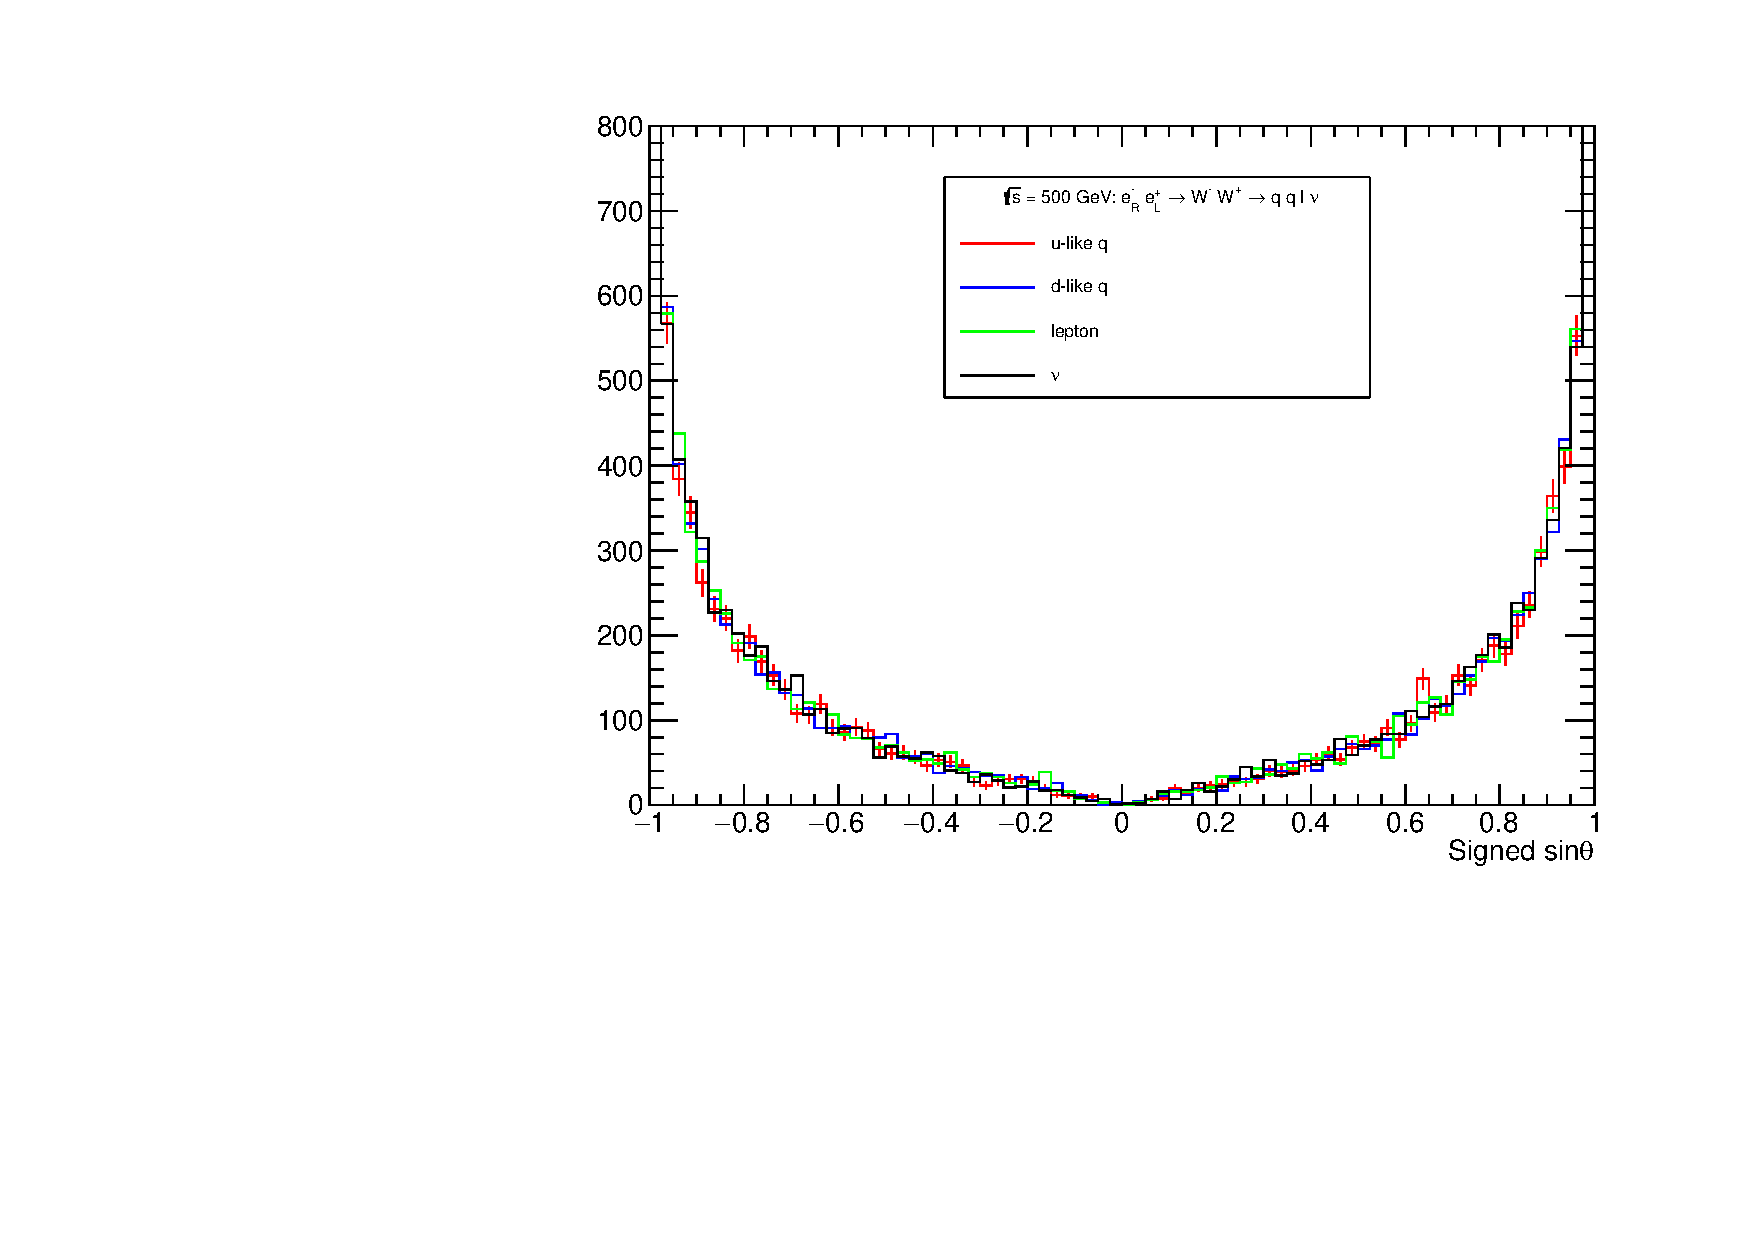
\includegraphics[width=0.48\textwidth]{hsRL.pdf}
\caption{The Signed sine of the polar angle of the true fermions with $\ell = \mu,\tau$. $100\%$ polarization for the initial state helicites. The sign of $sin\theta$ corresponds to the sign of $cos\theta$. As $sin\theta \rightarrow 0$ the fermion is forward in the detector but for $|sin\theta| \rightarrow 1$ the fermions become maximally transverse to the beam. In the LR configuration(Left) the charged lepton and down-like quark are scattered forward while the up-like quark and neutrino are ejected centrally into the detector. In the RL configuration(Right) all of the fermions are more centrally produced. }
\end{figure}

After a lepton candidate has been selected, the remaining particles in the system are expected to form the hadronically decaying W-boson. However, vector sum of the paricles  produces a distribution that is often in excess of the true hadonic mass. Variation between the true and measured mass naturally arise due to the mismeasurment of particles -- specically neutral hadrons, as well as particles lost beyond the acceptance range of the detector. Neither of these effects should create a systematic excess in the hadronic mass. The nature of the excess can be understood by through the kinematics of the WW in the LR and RL configurations shown in Figure \ref{fig:Epartition} and \ref{fig:fangles}. The highest yielding configuration, LR, typically has two fermions that are forward in the detector which both typically have a large fraction of the beam energy. These fermions are susceptible to pile-up scattering into the detector and mixing directly into the reconstructed jets. To combat effects of pile-up, jet clustering algorithms via FastJet\cite{fastjet} are used.  The standard approach for pileup mitigation is to use the kT algorithm\cite{kt} and tune the R parameter such that the pile-up particles associate with beam jets while the desired particles are not. With successful kT clustering the beam jets can be thrown away without damaging the reconstruction of the desired event. However, this approach only works well in events that are centrally produced.  The pile-up overlap in the forward topology with kT algorithm  based clustering leads to rejecting desired particles and severe undermeasuremnt of the the W mass. The solution to proper pileup mitigation is through the precise removal of foreign particles inside the reconstructed jets.  This can be achieved by using the standard JADE algorithm and mass based cut-off parameter $y_{cut} > y_{ij}$ where $y_{ij} = M_{ij}^2 / Q^2$ with $M_{ij}$ being the invariant mass of the pair of objects being combined and $Q^2$ being the visible energy in the $e^{+}e^{-}$ annihilation \cite{ycut}.  The mass of individually reconstructed jets can be controlled by tuning the $y_{cut}$ parameter. For large values, $y_{cut} =1\times10^{-3}$, a single massive jet is reconstructed. In the limit that $y_{cut}$ becomes infinitely small the number of jets reconstructed converges to the number of reconstructed particles.  The $y_{cut}$ value  chosen is the value that forms mini-jets that safely couple together hard and soft emissions from  the original quark jet while segregating pile-up into its own mini-jets. The mini-jets are then subjected to kinematic cuts that to maximize the pileup rejection and minimize the difference  between the true and measured hadronic W mass. The optimization is performed on the $100\%$ polarized LR signal muon dataset and the parameters used to select the best combination of $y_{cut}$ and mini-jet kinematic cuts are two statisical estimators from the distribution of $M_{qq}^{meas} - M_{qq}^{true}$. This binned mass difference distribution is created from the subset of mini-jets that arise from clustering with a given $y_{cut}$ and also pass some jet veto cuts $p_{Tjet} > x$ and $cos\theta_{jet} < y$. The estimators are the Full Width Half Maximum(FWHM) and the number of entries in the Mode.  
Using estimators calculated from a binned histogram creates unwanted sensitivity to bin size. To reduce sensitivity to binning, the mode is defined as the center of the bin with the most entries. The ``mode entries" is the number of entries in the mode bin plus the number of entries in the mode bins nearest neighbors. For the FWHM, the mass distribution is assumed to be monotonically decreasing around the half maxmimum. To create a continuous distribution of the FWHM across multiple optimization parameters the FWHM is weighted towards the bin center of the two bins around (above/below) the half maximum. The FWHM moves towards the bin center of the bin that is closer to the half maximum based on how close the both above/below bins are to the half maximum. The results of the optimization are shown in Figure \ref{fig:supmass} and various $y_{cut}$s are shown in comparison to the optimal configuration in Figure \ref{fig:supdiff}. The leading result uses $y_{cut} = 5\times 10^{-5}$, mini jet $P_T > 2$ GeV, and has no $\cos \theta$ requirement. 

\begin{figure}
    \centering
    \begin{minipage}{0.49\textwidth}
        \centering
        \label{fig:supdiff}
        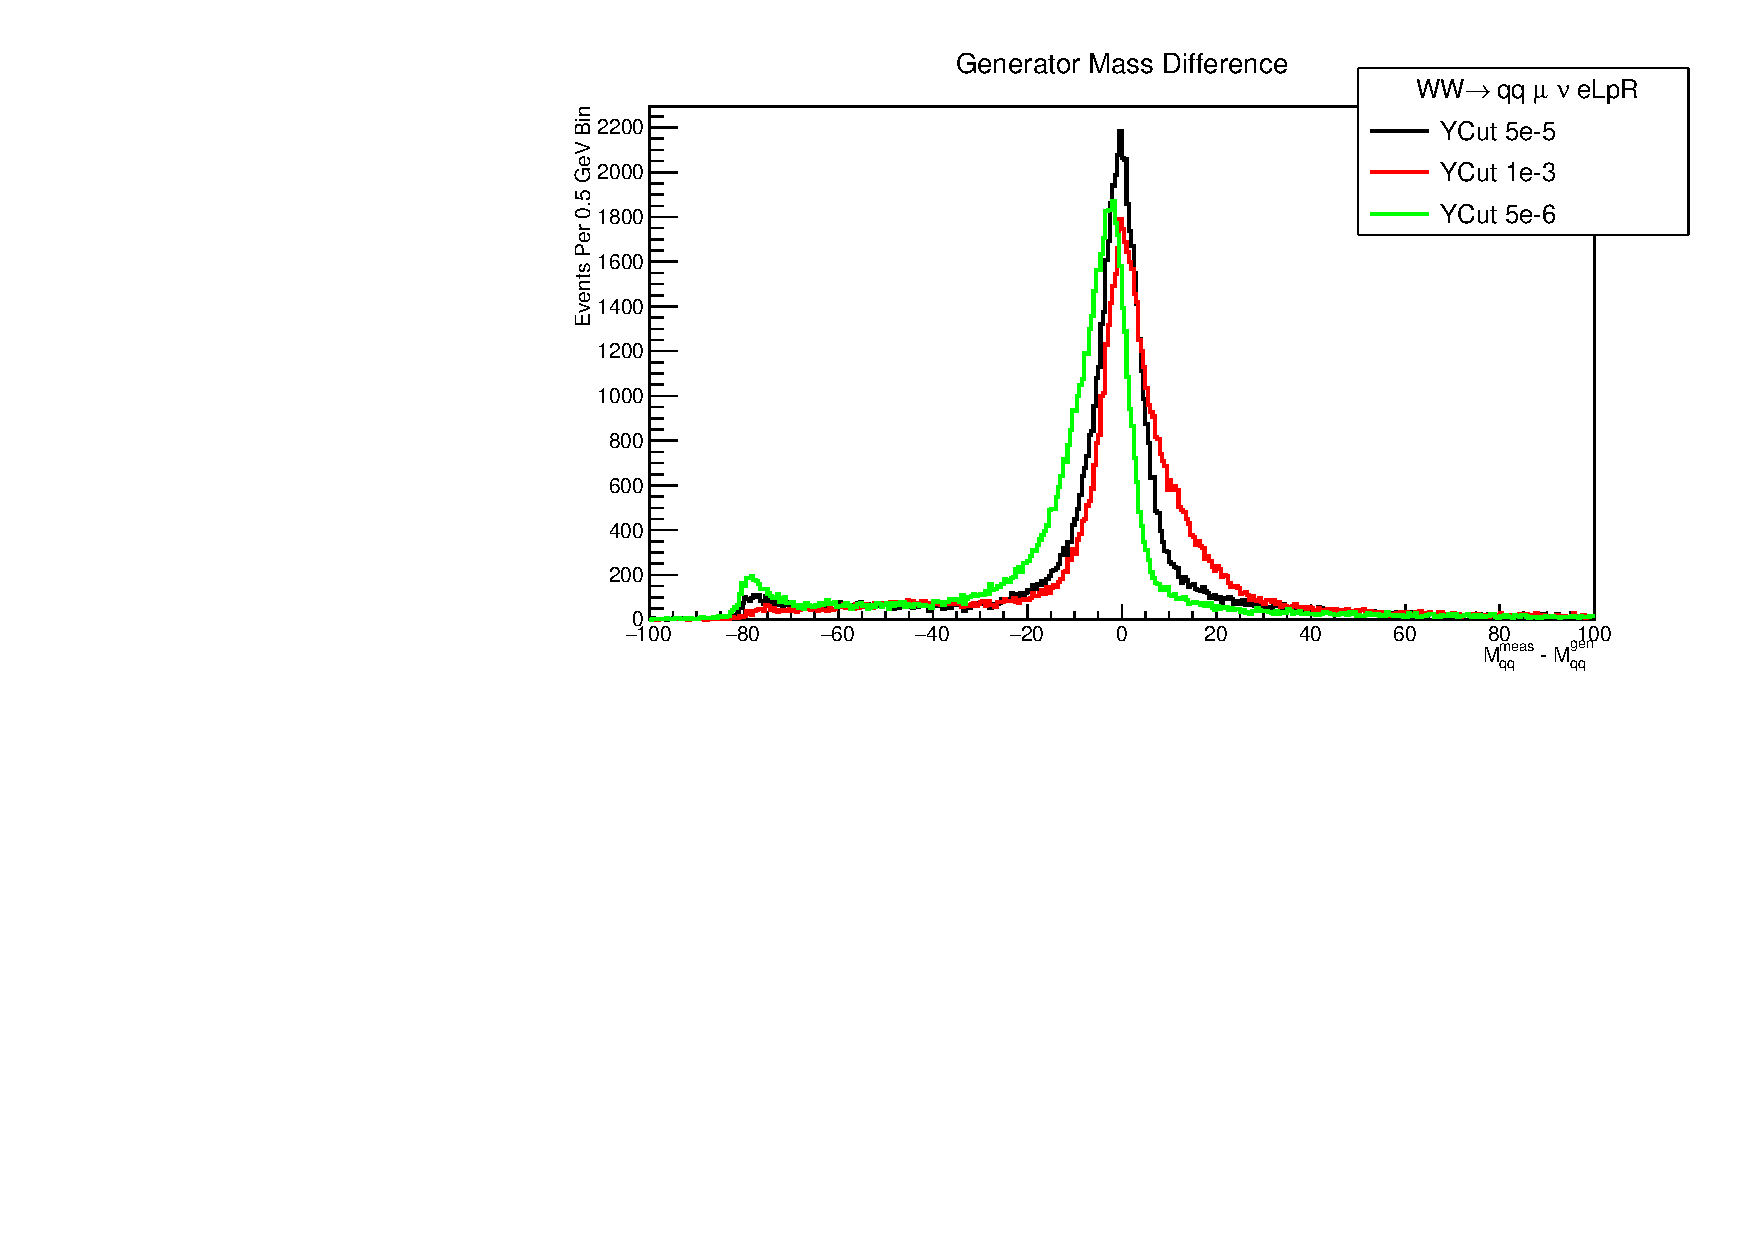
\includegraphics[width=0.99\textwidth]{SupDiff.pdf} % first figure itself
        \caption{Comparison of mass difference distributions with different $y_{cut}$ values and the same mini-jet cut $P_T > 2$. $y_{cut} = 1\times 10^{-3}$ results in massive jets that are not separated from pile-up and insensitive to small kinematic cuts. $y_{cut} = 5\times 10^{-5}$ has the best balance between jet clustering and mini-jet cuts. $y_{cut} = 5\times 10^{-6}$ yields a highly fragmented version of the jets where the mini-jets are not distinguishable from pile-up and are thrown out, resulting in the small peak around -80 GeV where the hadronic W is completely thrown out.  }
    \end{minipage}\hfill
    \begin{minipage}{0.49\textwidth}
        \centering
        \label{fig:supmass}
        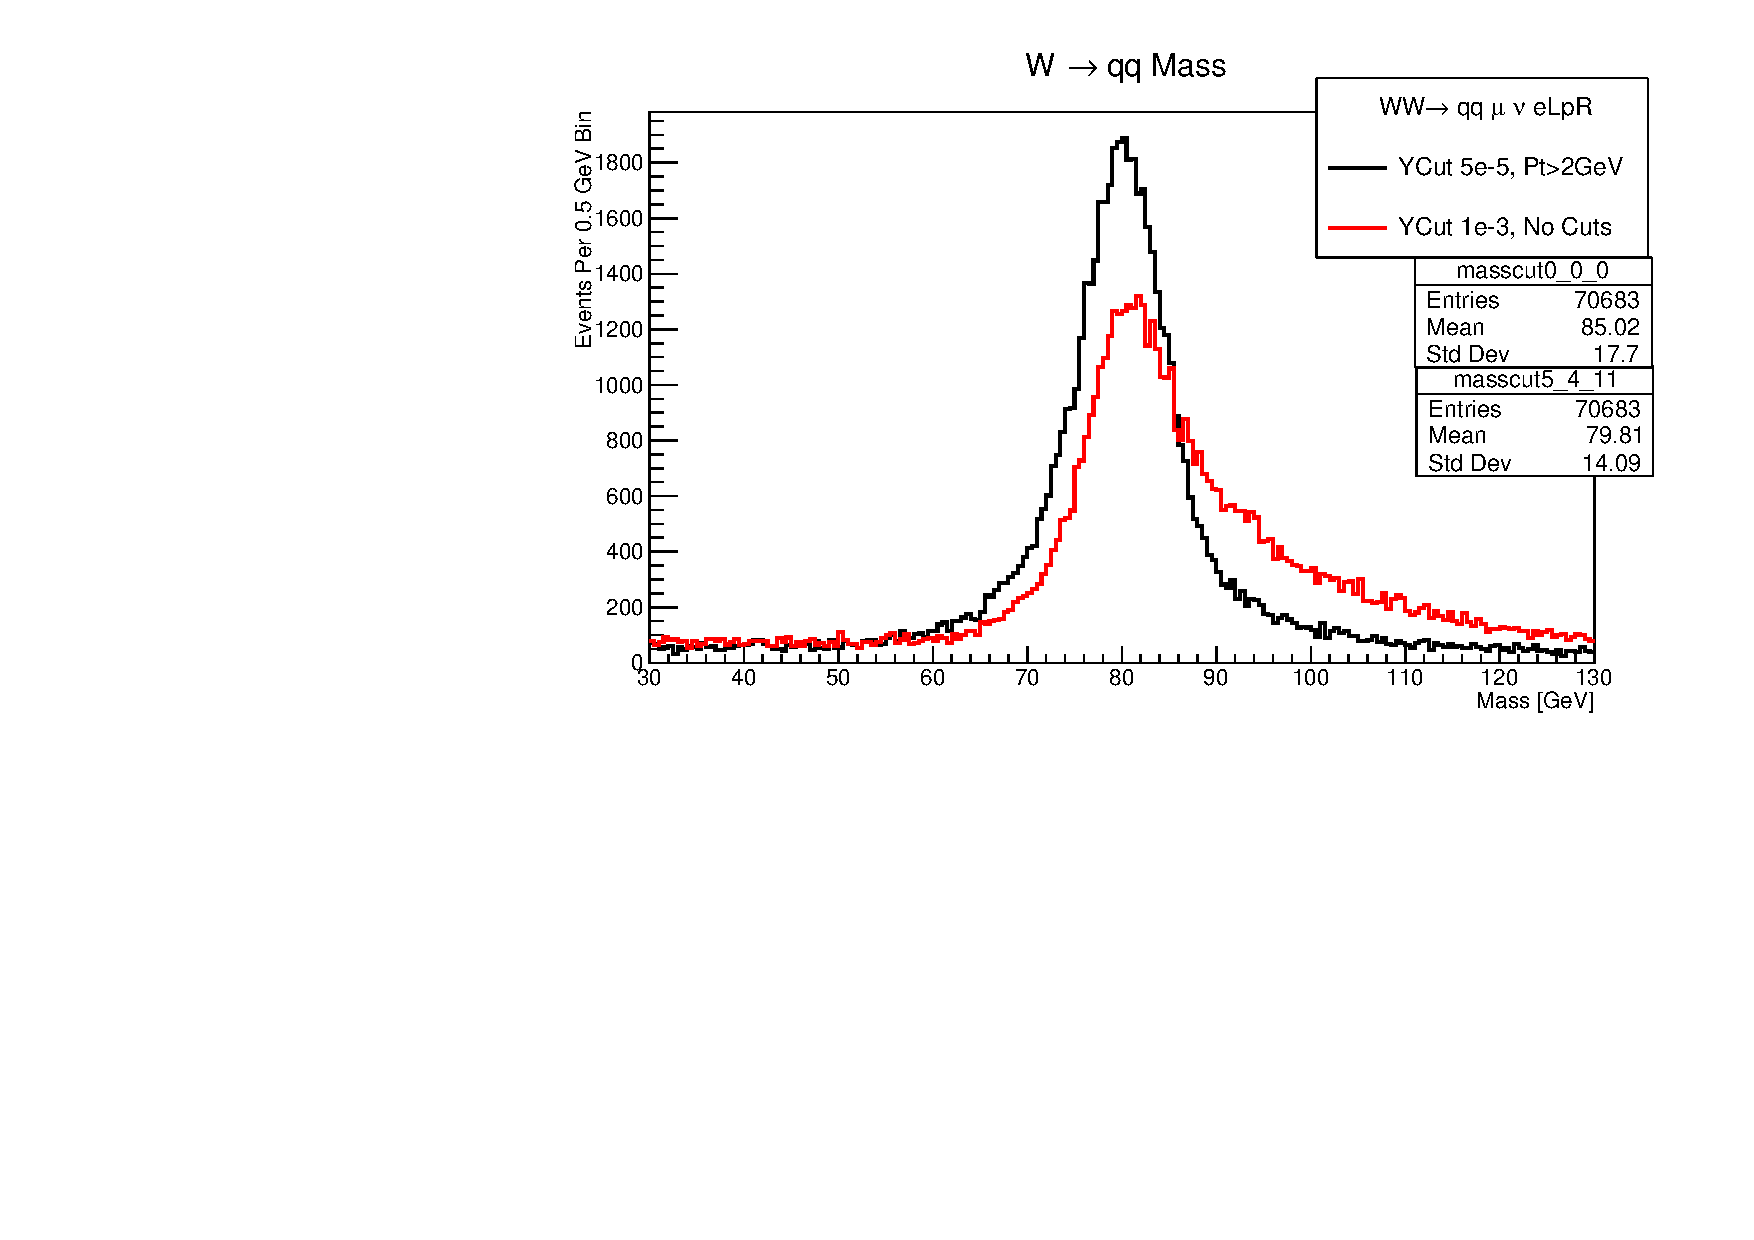
\includegraphics[width=0.99\textwidth]{SupMass.pdf} % second figure itself
        \caption{The increase of quality of the hadronic mass is shown between the red curve which is the raw hadronic system after lepton identification versus the black curve which is subjected to the pile-up mitigation with $y_{cut} = 5\times10^{-5}$ and mini jet $P_T > 2$ GeV. On average the excess in mass is reduced by $\approx 5$ GeV. }
    \end{minipage}
\end{figure}


\subsection{EventSelection}
\label{subsec:EventSelection}
The W-pair selection has been optimized for a Monte Carlo sample of 1600 $\text{fb}^{−1}$ with the $(-0.8,+0.3)$ beam scenario and is based on the selection in \ref{ivan}. The selection includes the full 2,4,6 fermion and Higgs SM background. The selection is performed with two independent subsets, a tight and loose selection. The tight selection uses the prompt $\mu$ cone to identify signal events that contain both prompt muons and electrons as wells as muon and electrons from tau decays. The tight selection is inefficient in collecting hadronic taus, so, the loose selection, using the inclusive tau cone, is designed to recover the efficiency of hadronic taus and problematic events. The selection criteria is as follows:
\begin{itemize}
\item N Leptons $\geq 1$
\item Track Multiplicity $> 10$  
\item Visible Pt $> 5$ GeV  
\item $E_{vis} < 500$ GeV 
\item $E_{com} > 100$ GeV
\item $40<M_{qq}<120$ GeV
\item  $-qcos\theta_W$
\item  $m^2_{\nu recoil} < 135,000 \, \, \text{GeV}^2$
\end{itemize}

\begin{figure}
 \centering
    \begin{minipage}{0.49\textwidth}
        \centering
        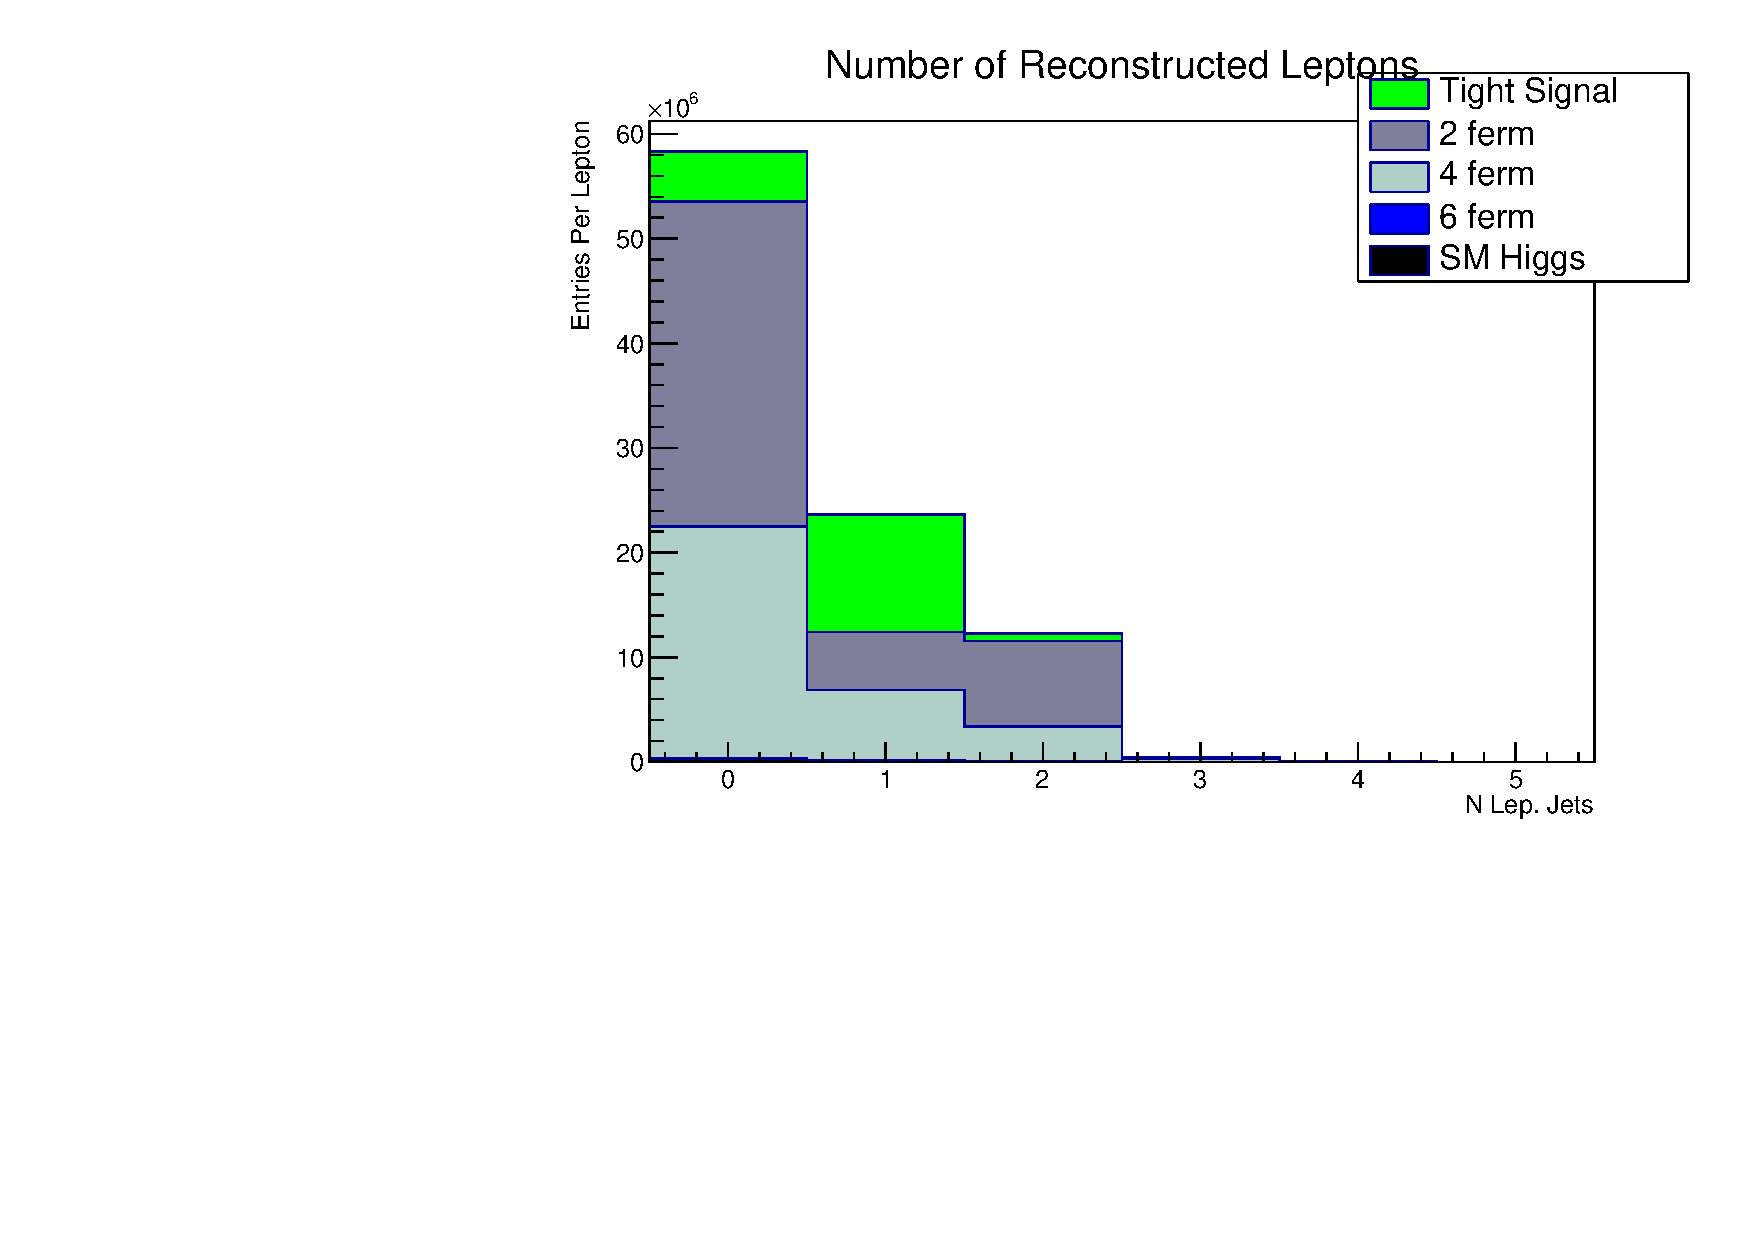
\includegraphics[width=0.99\textwidth]{nLepHist.pdf} % first figure itself
        \caption{first figure}
    \end{minipage}\hfill
    \begin{minipage}{0.49\textwidth}
        \centering
        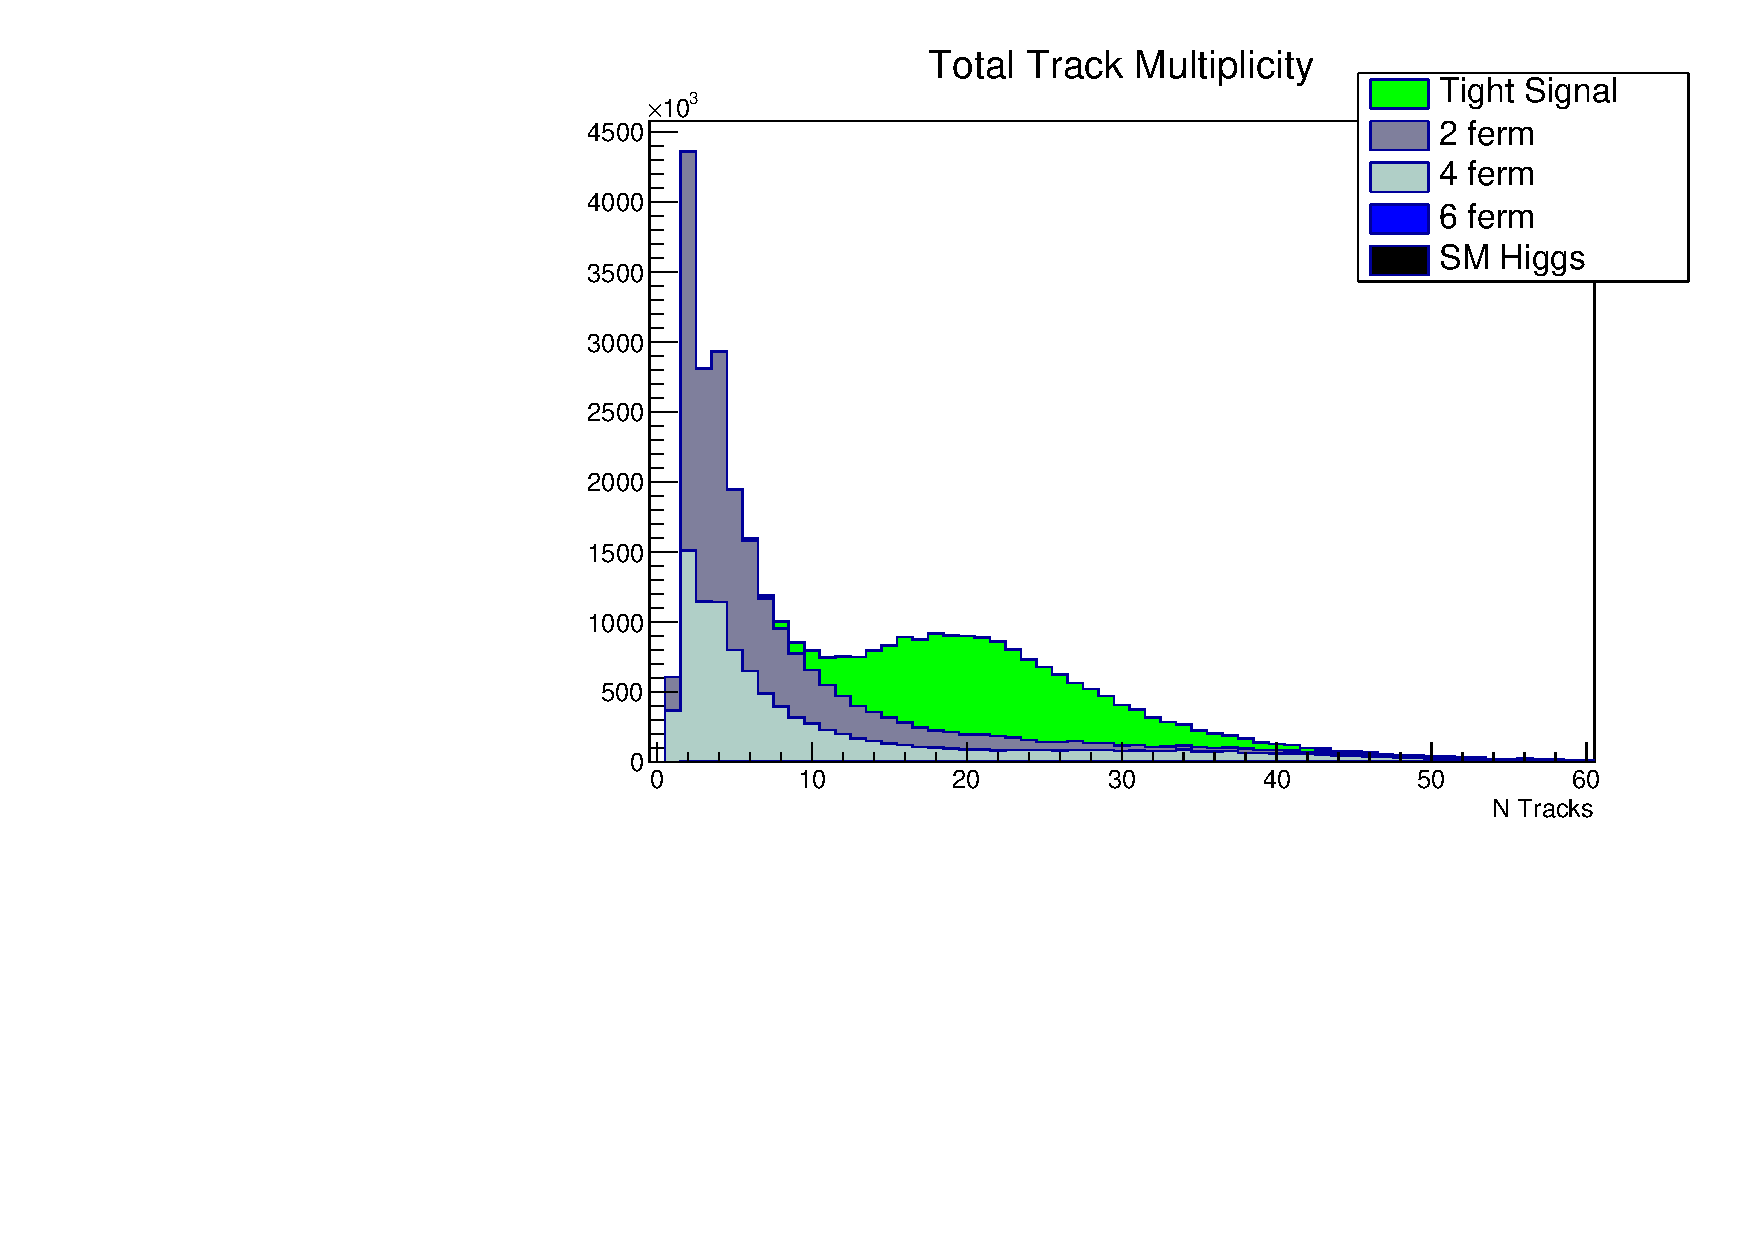
\includegraphics[width=0.99\textwidth]{ntracksHist.pdf} % second figure itself
        \caption{s}
     \end{minipage}
\end{figure}

\begin{figure}
 \centering
    \begin{minipage}{0.49\textwidth}
        \centering
        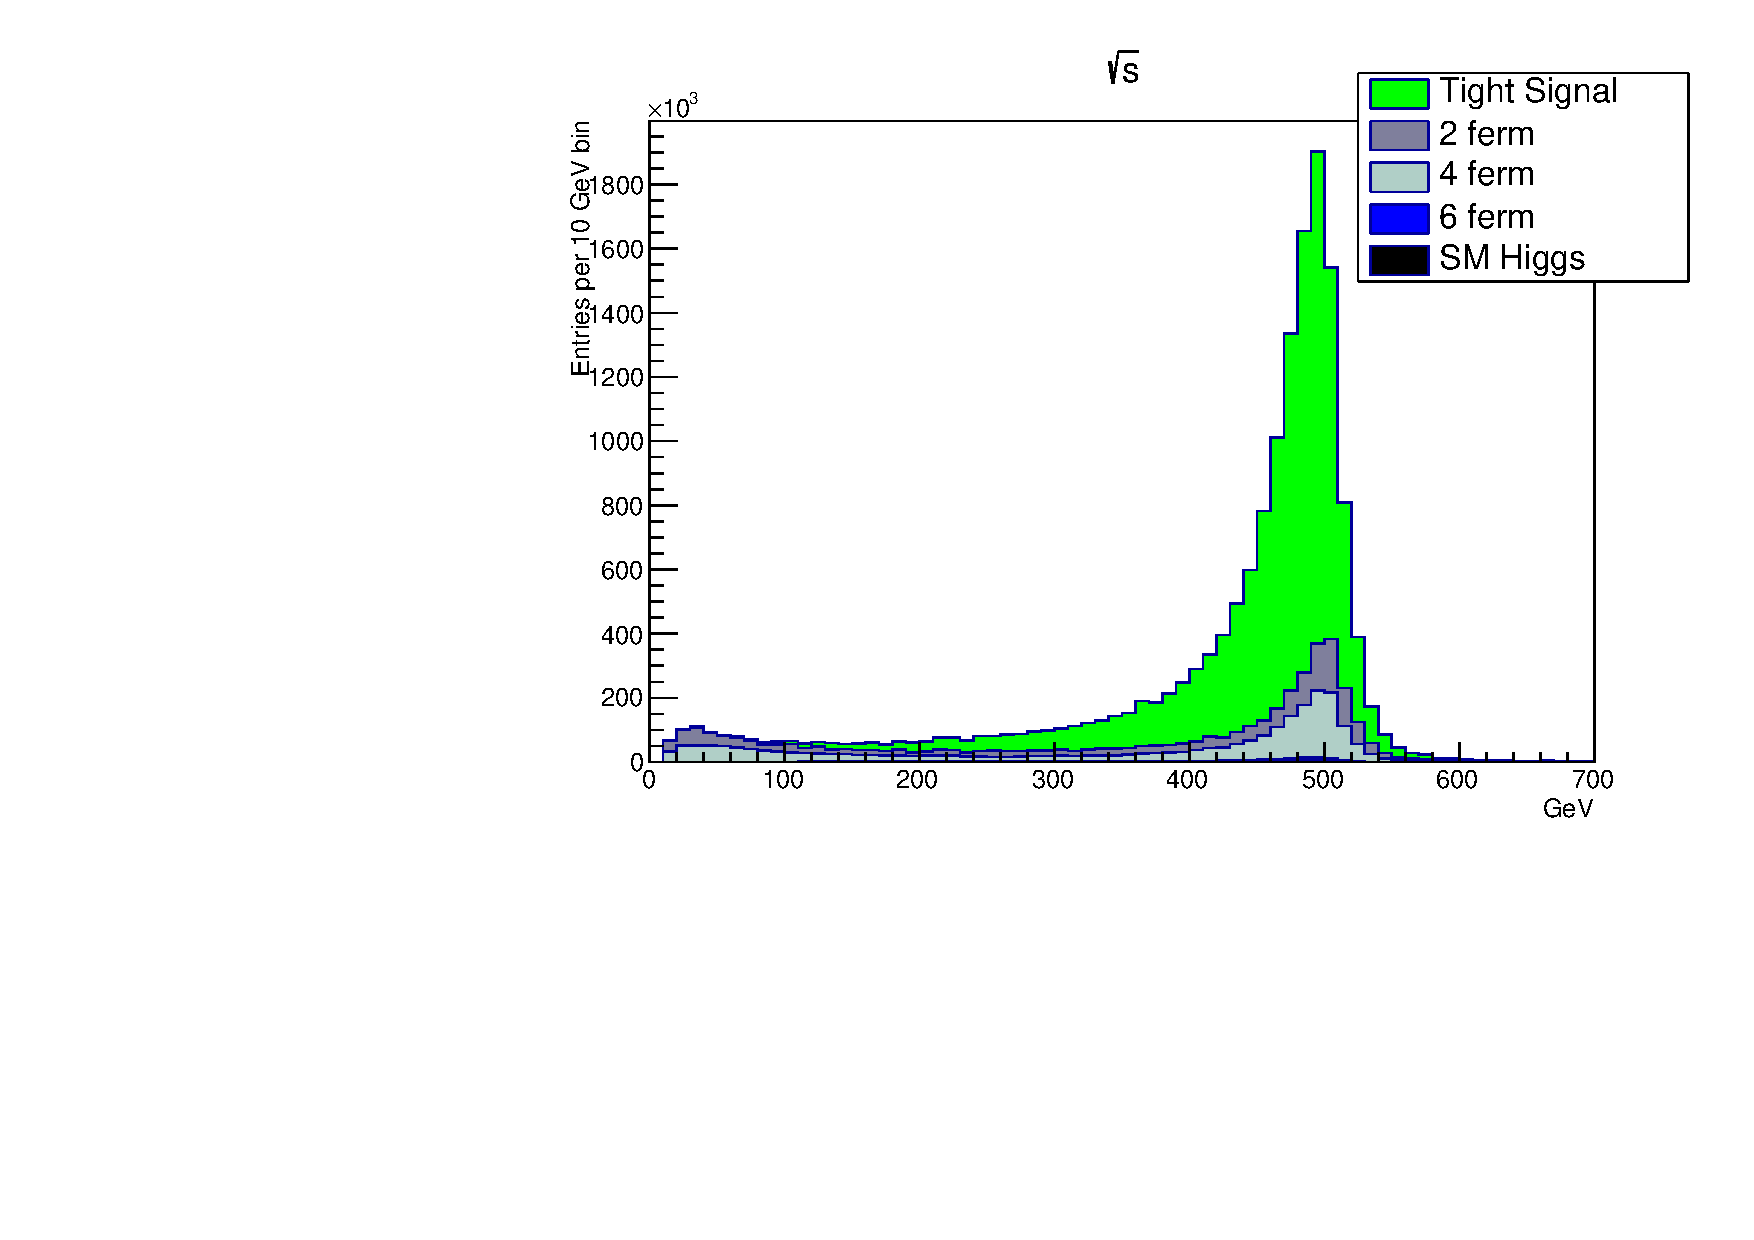
\includegraphics[width=0.99\textwidth]{EcomHist.pdf} % first figure itself
        \caption{first figure}
    \end{minipage}\hfill
    \begin{minipage}{0.49\textwidth}
        \centering
        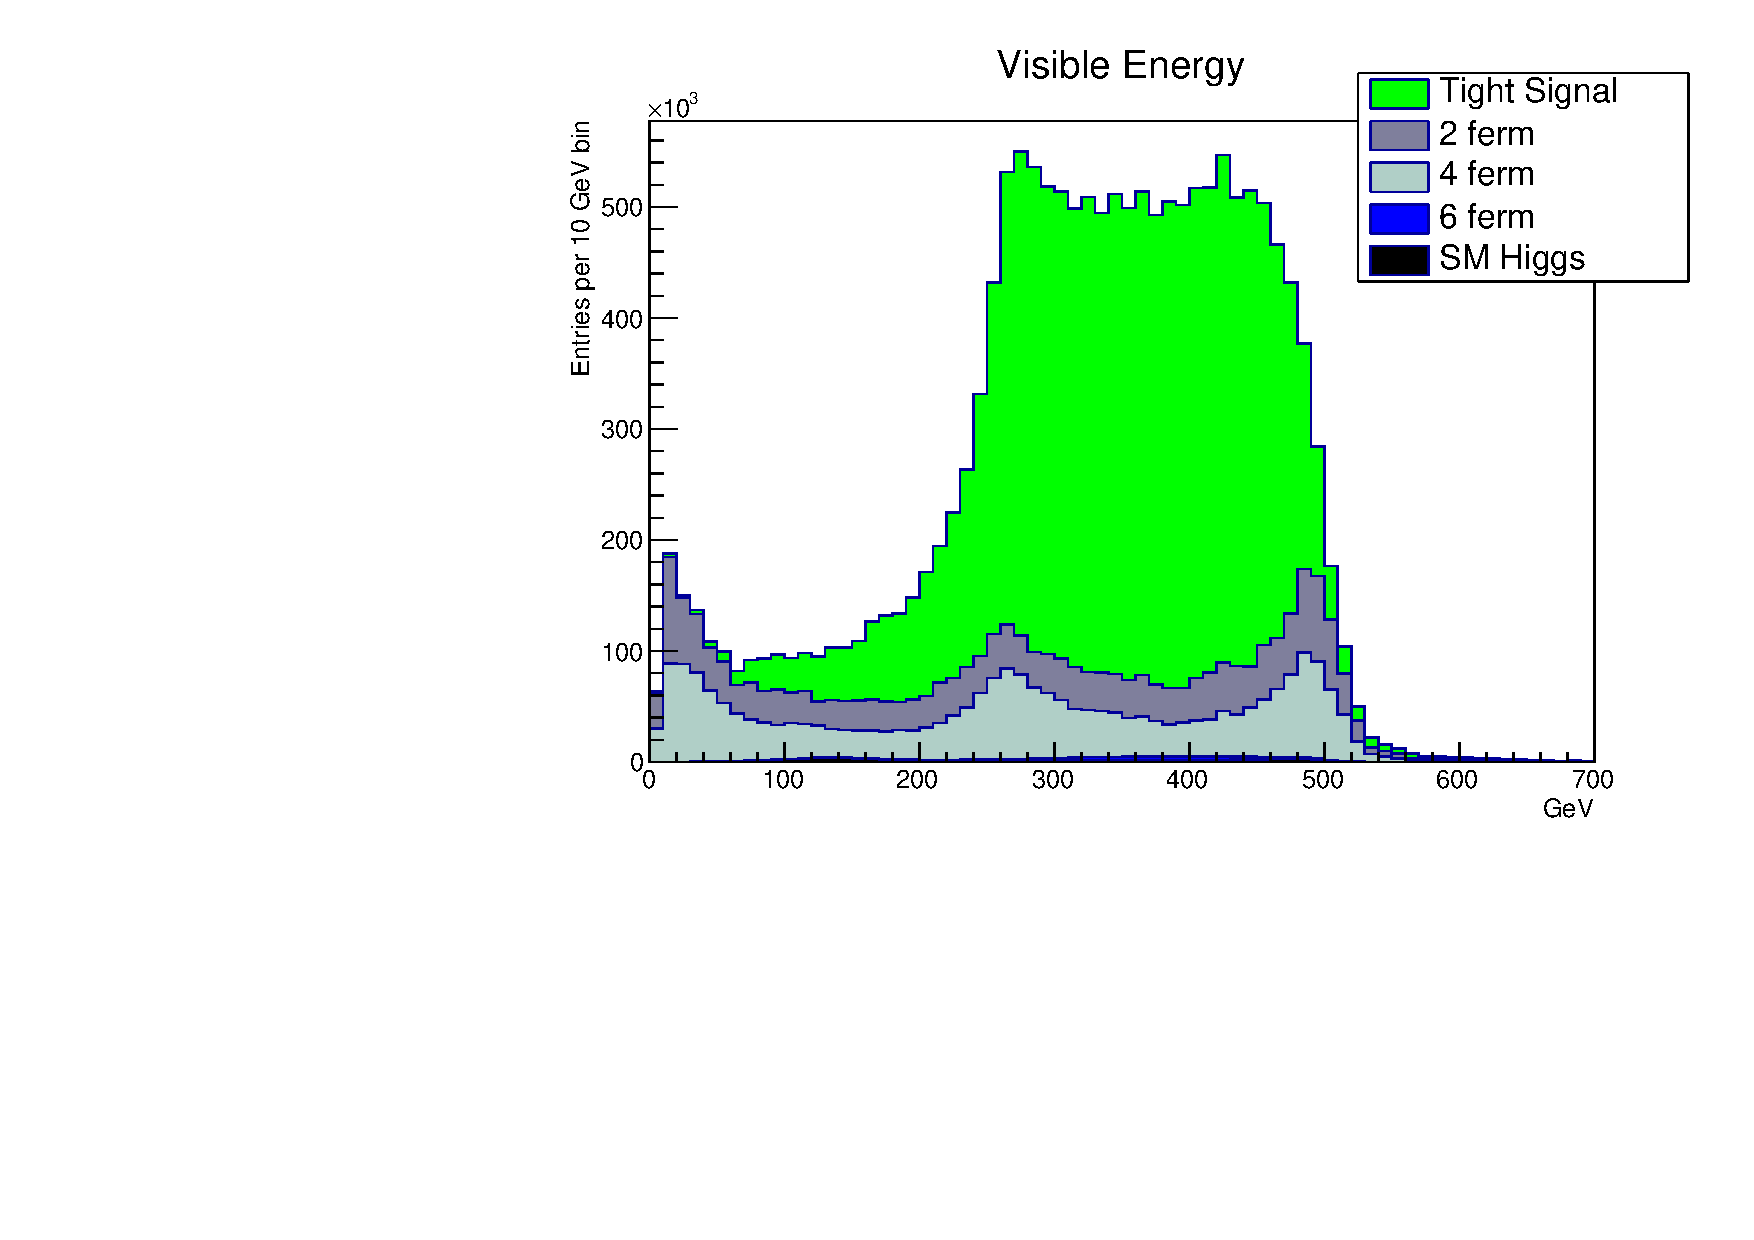
\includegraphics[width=0.99\textwidth]{EvisHist.pdf} % second figure itself
        \caption{s}
     \end{minipage}
\end{figure}
\begin{figure}
 \centering
    \begin{minipage}{0.49\textwidth}
        \centering
        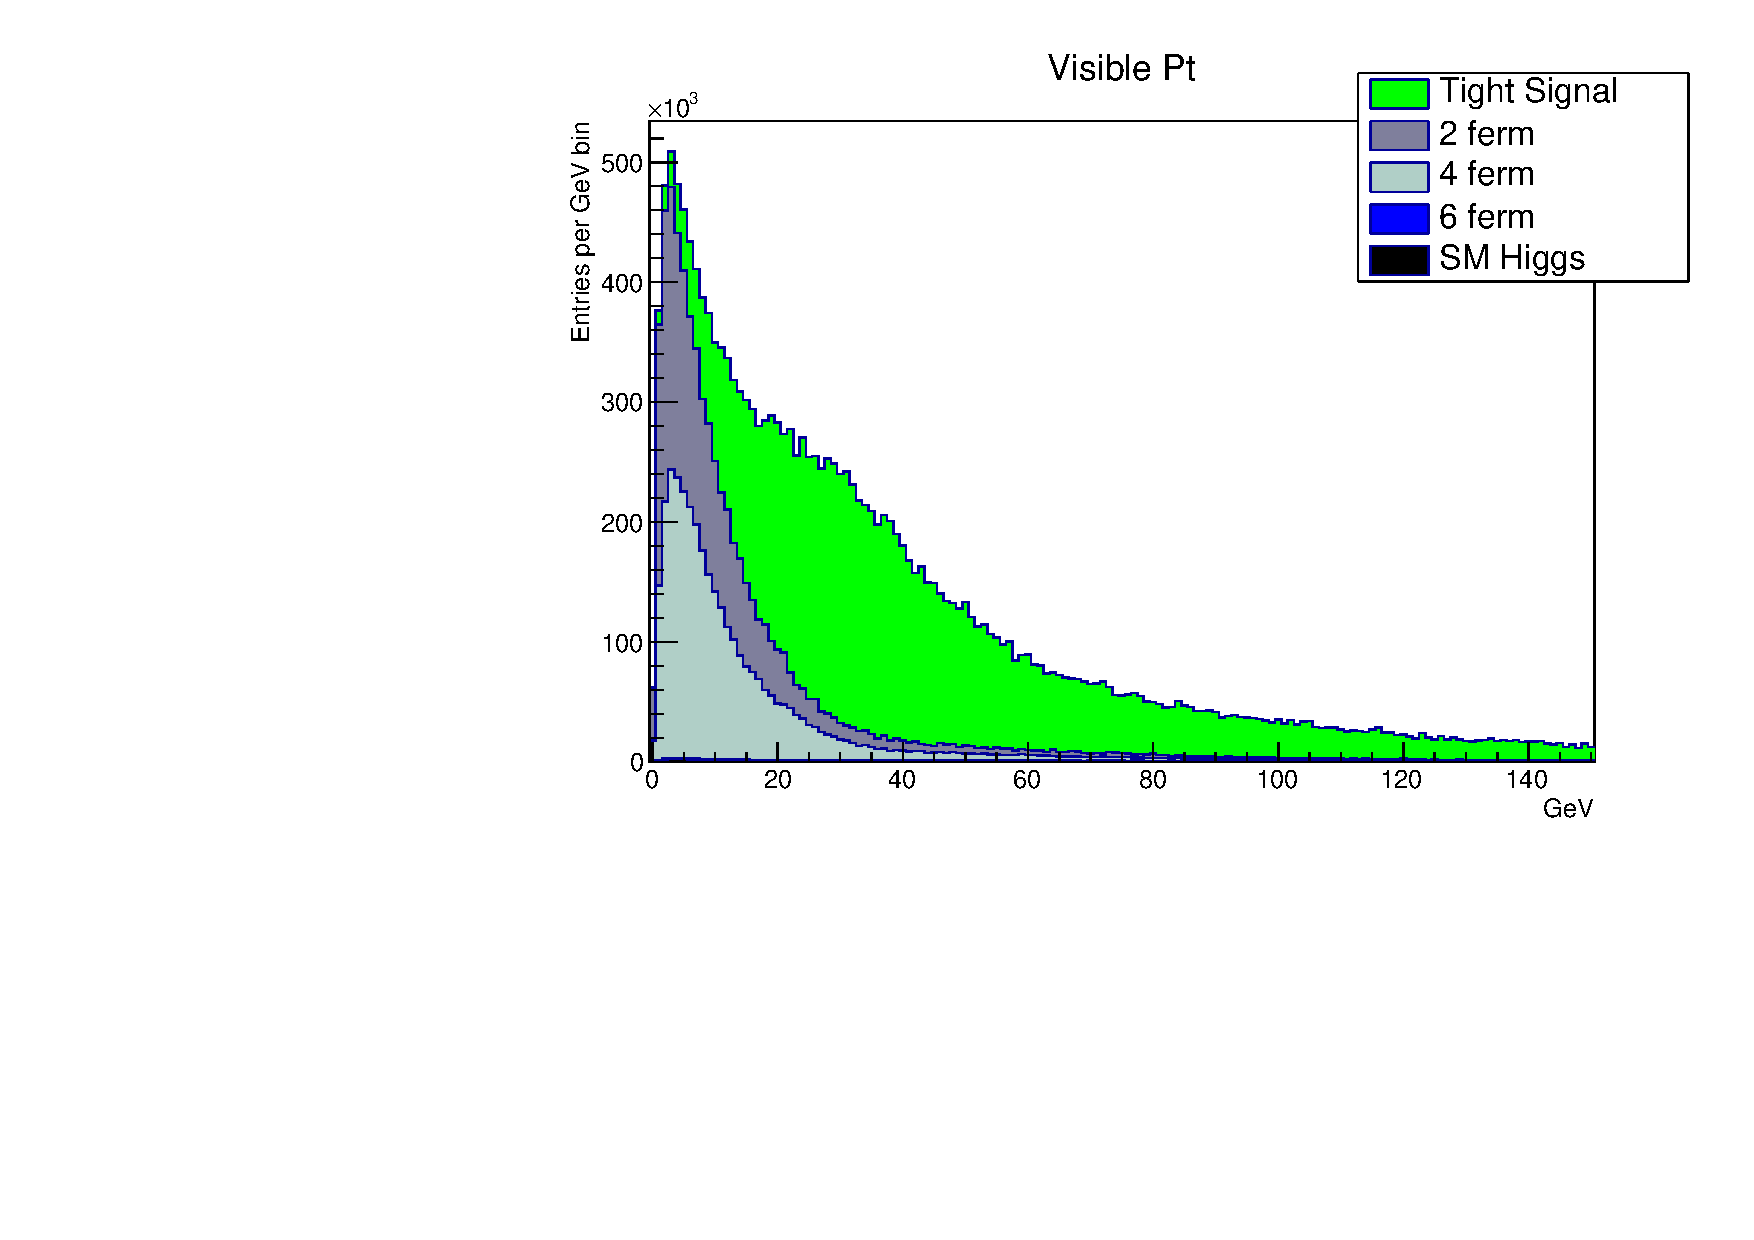
\includegraphics[width=0.99\textwidth]{PtvisHist.pdf} % first figure itself
        \caption{first figure}
    \end{minipage}\hfill
    \begin{minipage}{0.49\textwidth}
        \centering
        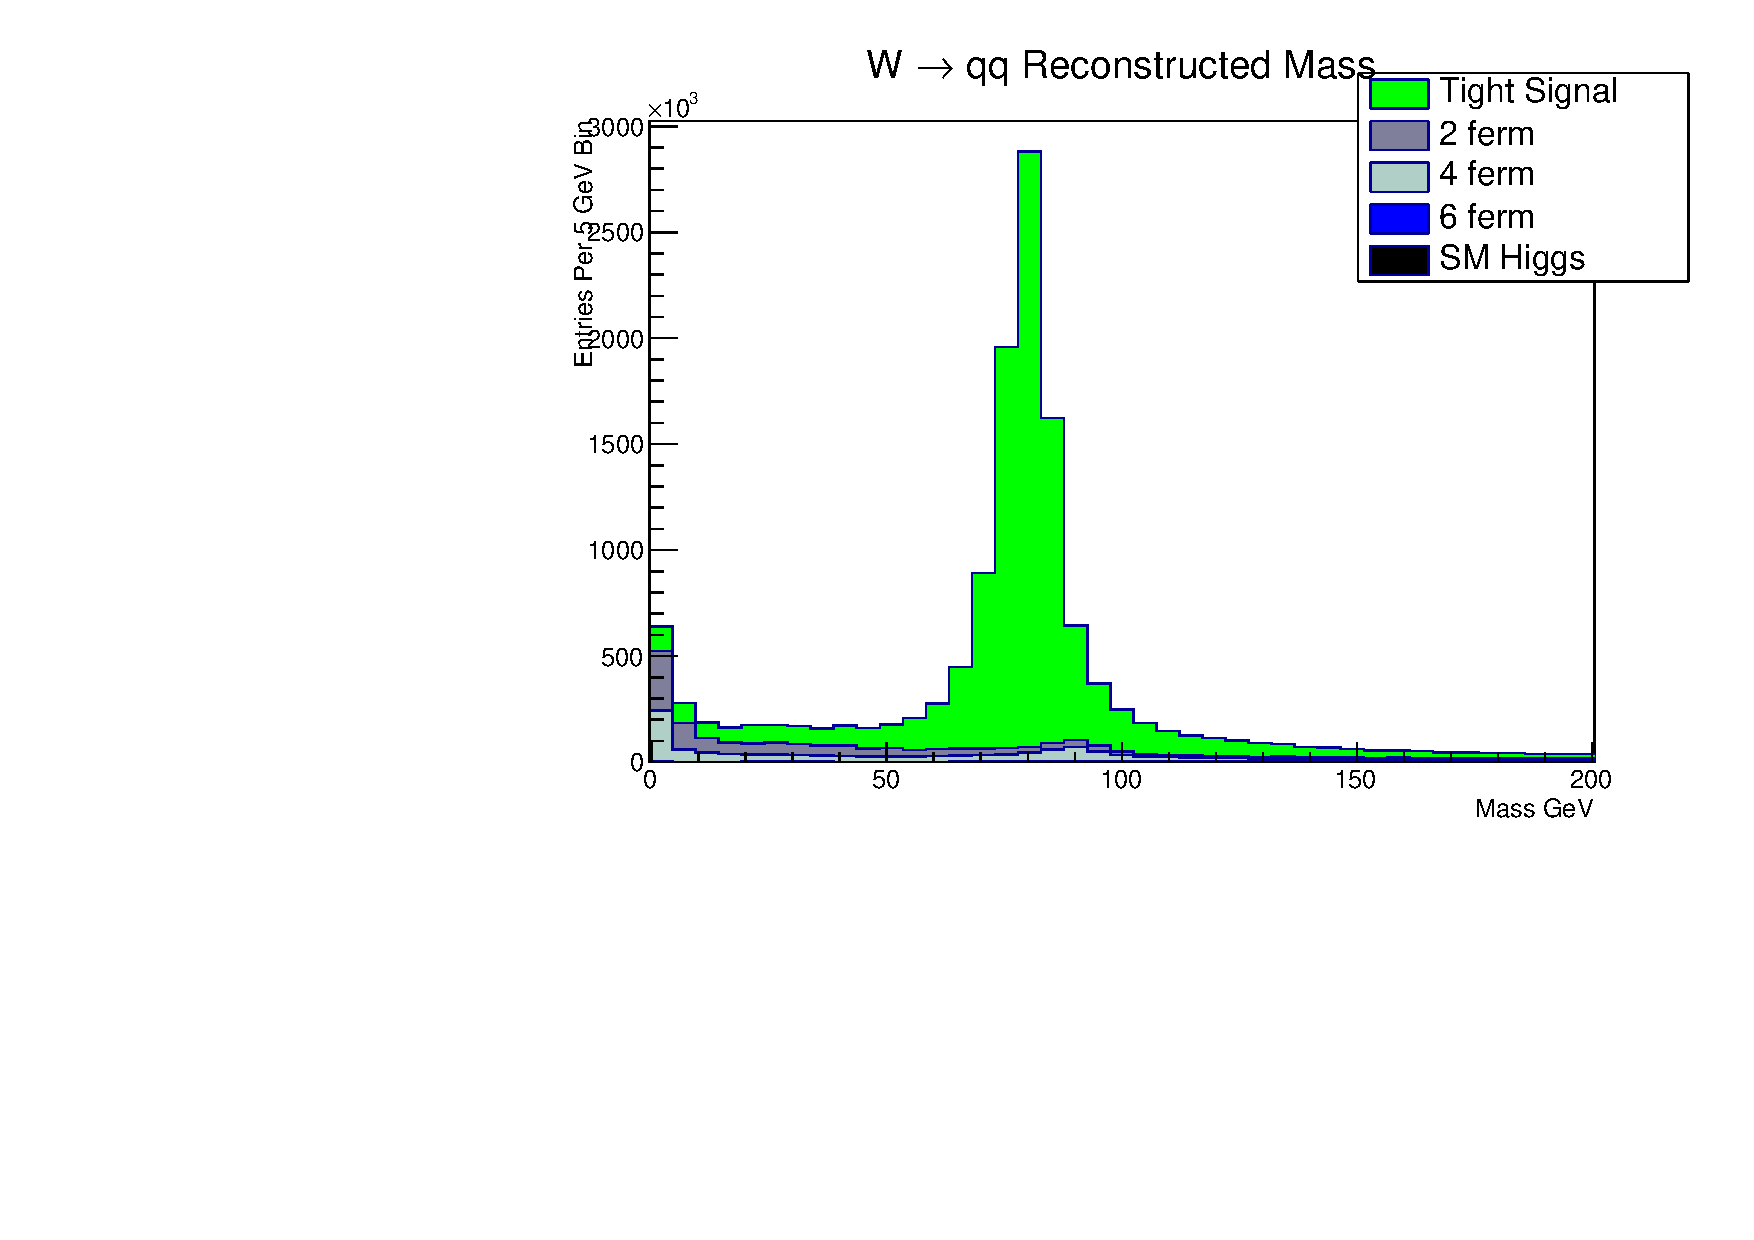
\includegraphics[width=0.99\textwidth]{mwhadHist.pdf} % second figure itself
        \caption{s}
     \end{minipage}
\end{figure}

\begin{figure}
 \centering
    \begin{minipage}{0.49\textwidth}
        \centering
        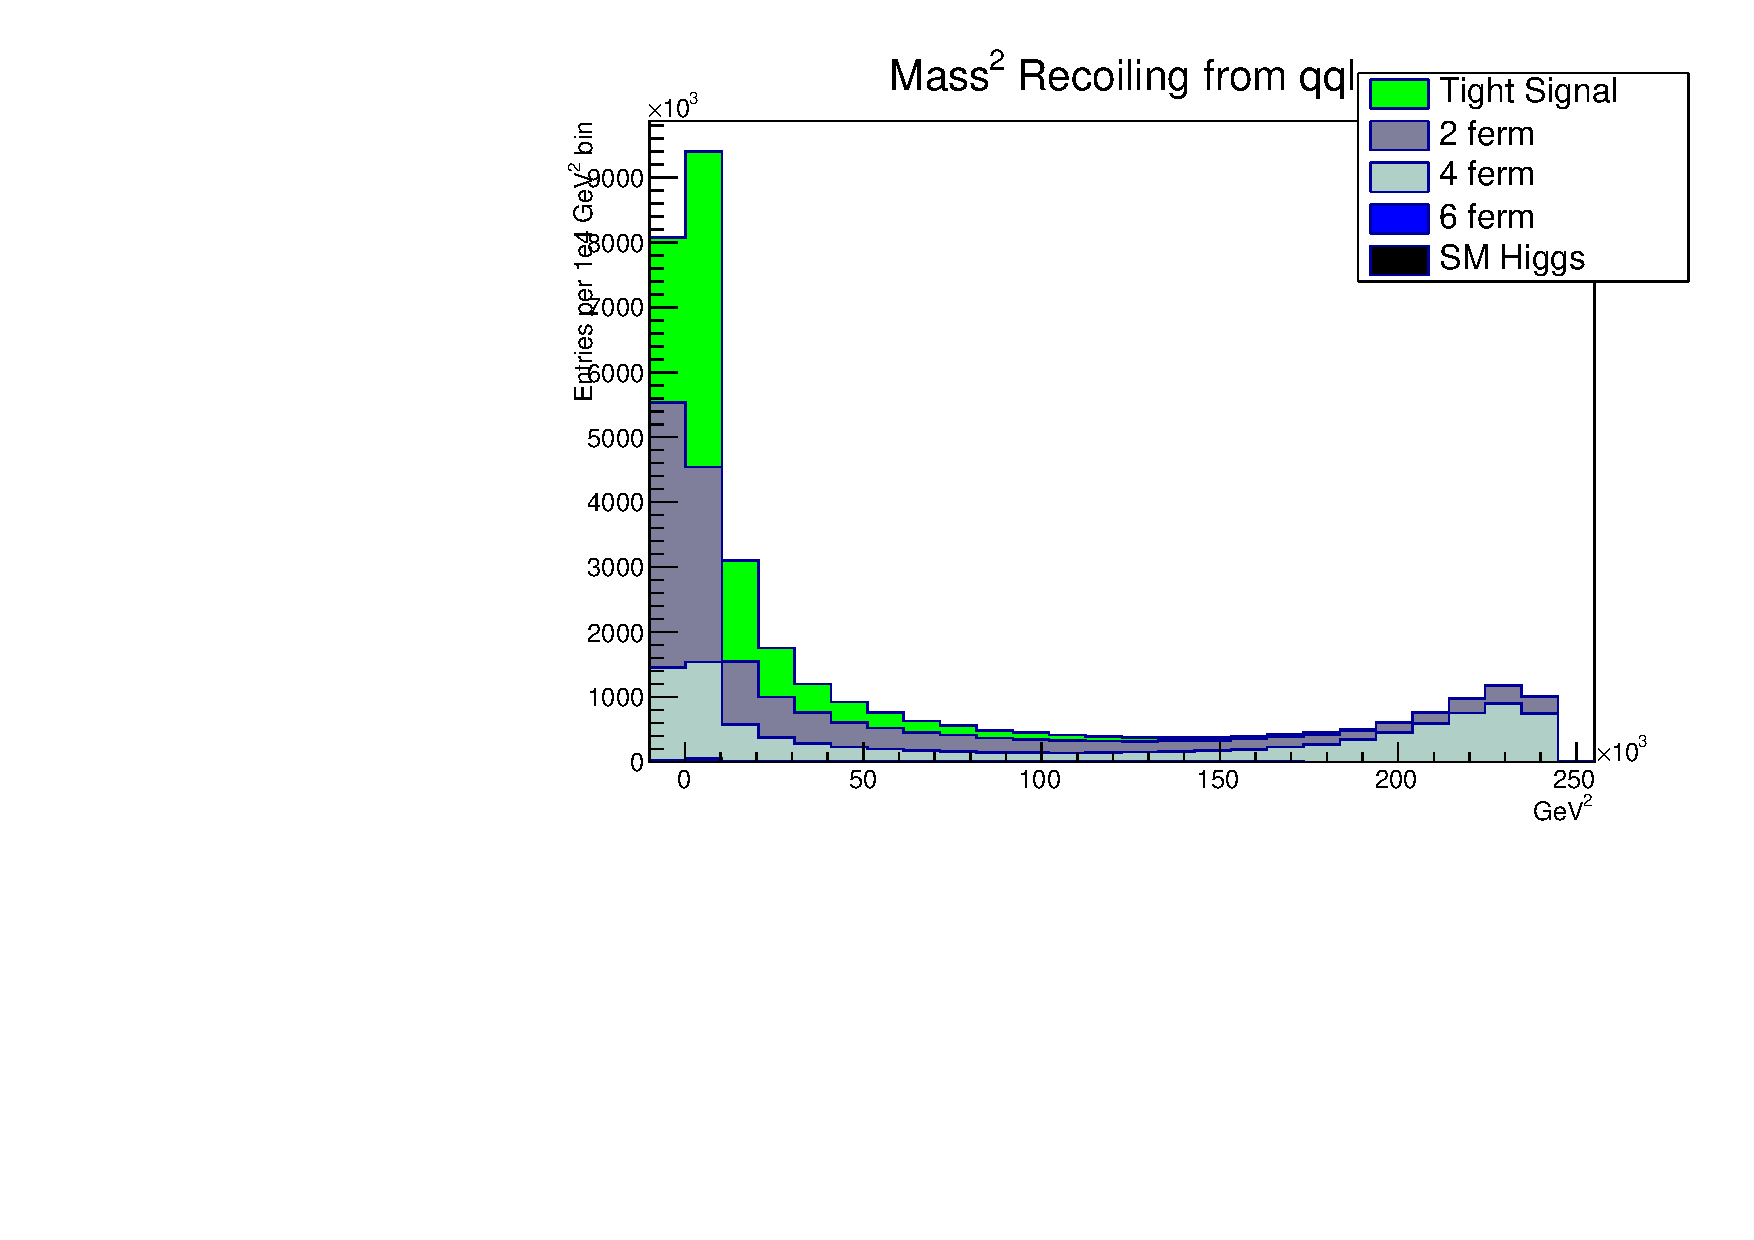
\includegraphics[width=0.99\textwidth]{vrecoilHist.pdf} % first figure itself
        \caption{first figure}
    \end{minipage}\hfill
    \begin{minipage}{0.49\textwidth}
        \centering
        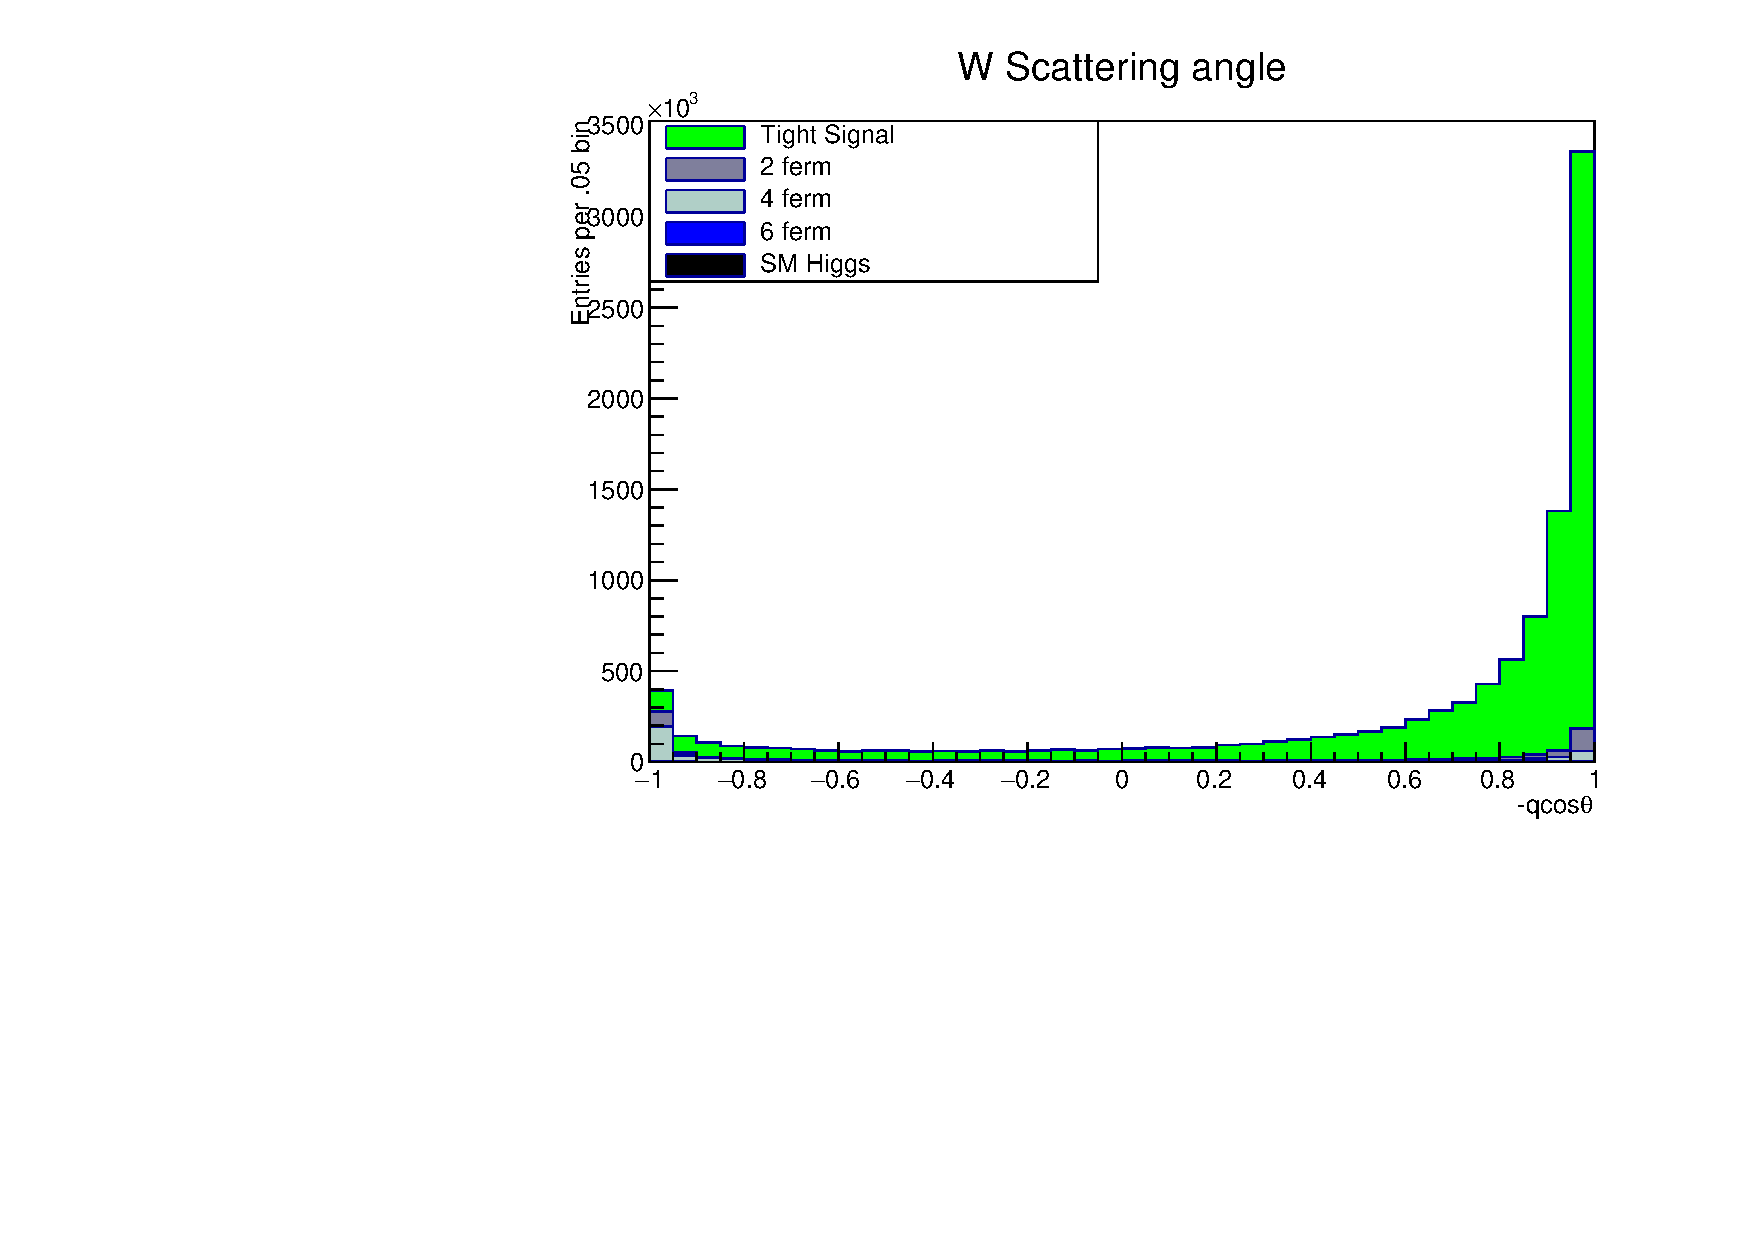
\includegraphics[width=0.99\textwidth]{qcostHist.pdf} % second figure itself
        \caption{s}\
     \end{minipage}
\end{figure}



   \begin{tabular}{|p{0.11\textwidth}|p{0.11\textwidth}p{0.11\textwidth}p{0.11\textwidth}p{0.11\textwidth}p{0.11\textwidth}p{0.11\textwidth}p{0.11\textwidth}p{0.1\textwidth}|}
\hline 
   & Prompt $\mu$ & Prompt $e$ & $\tau$ & Tot. Sig. & 2f & 4f & 6f & Higgs \\ \hline 
Base Evts &\num{3.87e+06 } & \num{3.89e+06 } & \num{3.90e+06} &\num{1.17e+07} & \num{4.22e+07} & \num{3.22e+07} & \num{2.14e+05} & \num{4.12e+05} \\ 

Lepton &\num{3.31e+06 } & \num{3.20e+06 } & \num{2.28e+06} &\num{8.78e+06} & \num{1.15e+07} & \num{1.18e+07} & \num{1.63e+05} & \num{1.15e+05} \\ 
 
$E_{vis}$ &\num{3.28e+06 } & \num{3.11e+06 } & \num{2.27e+06} &\num{8.67e+06} & \num{1.06e+07} & \num{1.15e+07} & \num{1.62e+05} & \num{1.11e+05} \\ 
 
N Tracks &\num{3.19e+06 } & \num{3.03e+06 } & \num{2.21e+06} &\num{8.43e+06} & \num{2.54e+06} & \num{2.59e+06} & \num{1.49e+05} & \num{8.89e+04} \\ 
 
$-qcos\theta$ &\num{3.18e+06 } & \num{3.01e+06 } & \num{2.18e+06} &\num{8.37e+06} & \num{2.19e+06} & \num{2.26e+06} & \num{1.44e+05} & \num{8.52e+04} \\ 
 
$M_{qq}$ $>$40 &\num{2.94e+06 } & \num{2.80e+06 } & \num{2.03e+06} &\num{7.77e+06} & \num{1.13e+06} & \num{1.33e+06} & \num{1.42e+05} & \num{7.56e+04} \\ 
 
$M_{qq}$ $<$120 &\num{2.72e+06 } & \num{2.57e+06 } & \num{1.83e+06} &\num{7.13e+06} & \num{5.68e+05} & \num{2.68e+05} & \num{2.02e+04} & \num{2.97e+04} \\ 
 
$E_{com}$ &\num{2.72e+06 } & \num{2.57e+06 } & \num{1.83e+06} &\num{7.13e+06} & \num{5.58e+05} & \num{2.65e+05} & \num{2.02e+04} & \num{2.96e+04} \\ 

Pt vis. &\num{2.69e+06 } & \num{2.55e+06 } & \num{1.81e+06} &\num{7.05e+06} & \num{3.21e+05} & \num{2.37e+05} & \num{2.01e+04} & \num{2.94e+04} \\ 

$m^2_{\nu recoil}$ &\num{2.69e+06 } & \num{2.54e+06 } & \num{1.80e+06} &\num{7.03e+06} & \num{2.93e+05} & \num{2.02e+05} & \num{1.94e+04} & \num{2.23e+04} \\ 
\hline 

 $\epsilon$ & $0.694 $ & $0.654 $ & $0.462$ &  $0.603 $ & $0.0069 $ & $0.00626 $ & $0.0905 $ & $0.0541 $ \\ 
 
 			& $\pm$0.002 & $\pm$0.002 & $\pm$0.003 & $\pm$0.002 & $\pm$ 0.0001 & $\pm$\num{8e-05} & $\pm$ 0.0002 & $\pm$0.0005 \\
\hline
\end{tabular}
\quad \quad \\
Loose selection with tau cone\\
\begin{tabular}{|p{0.11\textwidth}|p{0.11\textwidth}p{0.11\textwidth}p{0.11\textwidth}p{0.11\textwidth}p{0.11\textwidth}p{0.11\textwidth}p{0.11\textwidth}p{0.1\textwidth}|}
\hline 
   & Prompt $\mu$ & Prompt $e$ & $\tau$ & Tot. Sig. & 2f & 4f & 6f & Higgs \\ \hline 
Base Evts &\num{3.87e+06 } & \num{3.89e+06 } & \num{3.90e+06} &\num{1.17e+07} & \num{4.22e+07} & \num{3.22e+07} & \num{2.14e+05} & \num{4.12e+05} \\ 
 
Lepton &\num{3.36e+06 } & \num{3.30e+06 } & \num{2.82e+06} &\num{9.48e+06} & \num{1.30e+07} & \num{1.36e+07} & \num{1.77e+05} & \num{1.38e+05} \\ 

Tight Veto &\num{7.72e+04 } & \num{1.28e+05 } & \num{5.70e+05} &\num{7.76e+05} & \num{1.93e+06} & \num{2.15e+06} & \num{1.61e+04} & \num{3.12e+04} \\ 
 
$E_{vis}$ &\num{7.64e+04 } & \num{1.26e+05 } & \num{5.70e+05} &\num{7.72e+05} & \num{1.82e+06} & \num{1.94e+06} & \num{1.54e+04} & \num{3.02e+04} \\ 

N Tracks &\num{7.37e+04 } & \num{1.21e+05 } & \num{5.54e+05} &\num{7.49e+05} & \num{1.50e+06} & \num{1.64e+06} & \num{1.51e+04} & \num{2.71e+04} \\ 
 
$-qcos\theta$ &\num{6.30e+04 } & \num{1.12e+05 } & \num{5.32e+05} &\num{7.07e+05} & \num{1.11e+06} & \num{1.41e+06} & \num{1.45e+04} & \num{2.56e+04} \\ 
 
$M_{qq}$ $>$ 40 &\num{4.92e+04 } & \num{9.72e+04 } & \num{4.86e+05} &\num{6.33e+05} & \num{5.98e+05} & \num{1.30e+06} & \num{1.44e+04} & \num{2.33e+04} \\ 

$M_{qq}$ $<$ 120 &\num{4.04e+04 } & \num{7.81e+04 } & \num{4.16e+05} &\num{5.35e+05} & \num{2.58e+05} & \num{1.11e+05} & \num{1.11e+03} & \num{1.24e+04} \\ 
 
$E_{com}$ &\num{4.04e+04 } & \num{7.81e+04 } & \num{4.16e+05} &\num{5.34e+05} & \num{2.50e+05} & \num{1.10e+05} & \num{1.11e+03} & \num{1.24e+04} \\ 

Pt vis. &\num{4.00e+04 } & \num{7.74e+04 } & \num{4.12e+05} &\num{5.29e+05} & \num{1.17e+05} & \num{1.01e+05} & \num{1.11e+03} & \num{1.23e+04} \\ 
 
$m^2_{\nu recoil}$ &\num{3.94e+04 } & \num{7.70e+04 } & \num{4.07e+05} &\num{5.24e+05} & \num{1.02e+05} & \num{7.59e+04} & \num{1.02e+03} & \num{9.73e+03} \\ 
\hline 
 $\epsilon$ & $0.0102 $ & $0.0198 $ & $0.105 $ &  $0.0449 $ & $0.00241 $ & $0.00236 $ & $0.00474 $ & $0.0236 $ \\ 

  	     & $\pm 0.005$ & $\pm 0.0007$ & $\pm 0.002$ & $\pm 0.0007$ & $\pm$\num{3e-05} & $\pm$\num{4e-05} & $\pm$\num{7e-05} & $\pm$0.0002 \\

 \hline
 \end{tabular}



\begin{tabular}{|p{0.16\textwidth}|p{0.16\textwidth}p{0.16\textwidth}p{0.16\textwidth}|}
\hline 
 & Prompt $\mu$ O.S. & Prompt $e$ O.S. & Tau O.S. \\ \hline 
Base Evts &\num{5.78e+05 } & \num{3.88e+06 } & \num{5.70e+05}\\ 

Lepton &\num{5.11e+05 } & \num{2.27e+06 } & \num{3.42e+05}\\ 
 
$E_{vis}$ &\num{5.08e+05 } & \num{2.25e+06 } & \num{3.41e+05}\\ 

N Tracks &\num{4.95e+05 } & \num{2.19e+06 } & \num{3.35e+05}\\ 
 
$-qcos\theta$ &\num{4.94e+05 } & \num{2.10e+06 } & \num{3.31e+05}\\ 
 
$M_{qq}$ $>$ 40 &\num{4.67e+05 } & \num{2.01e+06 } & \num{3.14e+05}\\ 

$M_{qq}$ $<$ 120 &\num{3.44e+05 } & \num{1.81e+06 } & \num{2.39e+05}\\ 
 
$E_{com}$ &\num{3.44e+05 } & \num{1.81e+06 } & \num{2.39e+05}\\ 

 Pt vis.&\num{3.40e+05 } & \num{1.80e+06 } & \num{2.36e+05}\\ 
 
$m^2_{\nu recoil}$ &\num{3.40e+05 } & \num{1.76e+06 } & \num{2.34e+05}\\ 
\hline 
 $\epsilon$ & $0.588 \pm 0.006$ & $0.454 \pm 0.001$ & $0.411 \pm 0.006$ \\  \hline
\end{tabular}



  \begin{tabular}{|p{0.16\textwidth}|p{0.16\textwidth}p{0.16\textwidth}p{0.16\textwidth}|}
\hline 
   & Prompt $\mu$ O.S. & Prompt $e$ O.S. & Tau O.S. \\ \hline 
Base Evts &\num{5.78e+05 } & \num{3.88e+06 } & \num{5.70e+05}\\ 

Lepton &\num{5.15e+05 } & \num{2.47e+06 } & \num{4.26e+05}\\ 
 
Tight Veto &\num{8.18e+03 } & \num{2.61e+05 } & \num{8.83e+04}\\ 
 
$E_{vis}$ &\num{7.87e+03 } & \num{2.61e+05 } & \num{8.83e+04}\\ 
 
N Tracks &\num{7.57e+03 } & \num{2.48e+05 } & \num{8.63e+04}\\ 
 
$-qcos\theta$ &\num{6.97e+03 } & \num{2.31e+05 } & \num{8.15e+04}\\ 
 
$M_{qq}$ $>$ 40 &\num{5.60e+03 } & \num{1.38e+05 } & \num{7.66e+04}\\ 
 
$M_{qq}$ $<$ 120 &\num{3.63e+03 } & \num{1.20e+05 } & \num{4.82e+04}\\ 
 
$E_{com}$ &\num{3.63e+03 } & \num{1.18e+05 } & \num{4.82e+04}\\ 

Pt vis. &\num{3.63e+03 } & \num{1.18e+05 } & \num{4.77e+04}\\ 
 
$m^2_{\nu recoil}$ &\num{3.63e+03 } & \num{9.15e+04 } & \num{4.73e+04}\\ 
\hline 
 $\epsilon$ & $0.006 \pm 0.001$ & $0.0236 \pm 0.0005$ & $0.083 \pm 0.004$ \\ \hline


\end{tabular} \\
%\subsection{Lepton ID}
%\label{subsec:Lepton_ID}

%\subsection{Pileup mitigation}
%\label{subsec:Pileup_mitigation}

%\subsection{EventSelection}
%\label{subsec:EventSelection}
%------------------------------------------------------------

\section{Discussion and Conclusions}
\label{future_analysis}
%\input{future_analysis}

%------------------------------------------------------------

%\section{Conclusions}
%\label{sec:Conclusions}
%\input{Conclusions.tex}

%------------------------------------------------------------

\clearpage %uncomment to push bib to next page
\bibliography{mybib}{}
\bibliographystyle{abbrv}

\end{document}